\documentclass[12pt, a4paper]{report}

%Packages
\usepackage[utf8]{inputenc}
\usepackage{geometry}
\geometry{margin=1in}
\usepackage{graphicx}
\usepackage[hidelinks]{hyperref}
\usepackage{float}
\usepackage{titlesec}
\usepackage{xcolor}
\usepackage{booktabs}
\usepackage{fancyhdr}
\usepackage{pdfpages}
\usepackage{longtable}
\usepackage{csvsimple}
\usepackage{etoolbox}
\usepackage{array}

%Custom Environments for Safety
\usepackage{tcolorbox}
\newtcolorbox{warning}{colback=orange!5!white,colframe=orange!75!black,title=WARNING}
\newtcolorbox{caution}{colback=yellow!5!white,colframe=yellow!85!black,title=CAUTION}
\newtcolorbox{danger}{colback=red!5!white,colframe=red!75!black,title=DANGER}
\newtcolorbox{notice}{colback=blue!5!white,colframe=blue!85!black,title=NOTICE}


%Header/Footer Setup
\pagestyle{fancy}
\fancyhead[L]{Glovebox Closure Mechanism}
\fancyhead[R]{User Manual v1.0}

%Title Page Data
\title{\textbf{LANL Glovebox Closure Mechanism}\\ \Large New Mexico Institute of Mining and Technology \\ User Manual}
\author{Aaron Madrid, Andrew Bemis,\\Alexander Watts, Alexander Schneller}
\date{\today}

\begin{document}

%Front Matter
\maketitle

\begin{abstract}
The purpose of this user manual is to serve as a user manual for the usage of the Glovebox Closure Mechanism designed by New Mexico Institute of Mining and Technology (NMT) for usage by the Los Alamos National Labs (LANL) on their gloveboxes. The mecahnism is designed to reducex the airflow into a glovebox in the event of a glove breach or an internal fire. 
\end{abstract}

\tableofcontents
\listoffigures
\listoftables

% Chapter 1: Introduction
\chapter{Introduction}

This manual provides operational guidance, safety procedures, inspection requirements, and system specifications for the Glovebox Closure Mechanism developed for Los Alamos National Laboratory (LANL) by the New Mexico Tech Mechanical Engineering Design Team. The purpose of this document is to ensure safe installation, inspection, and operation of the mechanism in conjunction with existing LANL safety protocols.

This manual is not intended to replace institutional safety policies or fire protection systems. Rather, it provides detailed instructions specific to this closure mechanism and its installation and inspection. 

Even the most advanced safety mechanism is ineffective without proper inspection, maintenance, and responsible operation.

\section{Intended Use}

The closure mechanism is designed to reduce airflow into a glovebox in the event of elevated temperature conditions indicative of fire. The glovebox operates under negative pressure, which may draw external oxygen into the enclosure during a fire or glove port failure. The system is intended to:
    \begin{itemize}
        \item Detect elevated temperatures through mechanical actuation 
        \item Engage a passive closure system 
        \item Reduce air ingress 
        \item Limit combustion intensification 
    \end{itemize}
The mechanism is not intended to serve as a primary fire suppression system.

\section{Limitations of Use}
This mechanism:
\begin{itemize}
        \item Does not extinguish fires.
        \item Does not replace fire suppression systems.
        \item Is not rated for structural containment of explosions.
        \item Must not be modified without engineering approval.
    \end{itemize}
Operation outside specified temperature, environmental, or mechanical limits may result in failure to actuate or unintended actuation.

\section{Design Specifications}
    \begin{table}[H]
        \centering
        \begin{tabular}{@{}ll@{}}
        \toprule
        Parameter & Specification \\ \midrule
        Final flow & $< 5$ CFM \\
        Actuation Time & $< 5$ min \\
        Actuation Temperature & $180^\circ$F \\
        Max Temperature & $1700^\circ$F \\
        Sensor Type & Mechanical Actuation \\ \bottomrule
        \end{tabular}
        \caption{General Specifications}
    \end{table}

\section{Primary Subsystems}
There are four primary subsystems; the Arm Cuff, the Heat Fuse, the Actuation Mechanism, and the Secondary Closure as shown in Figure \ref{fig:subsections}

\begin{figure}[H]
    \centering
    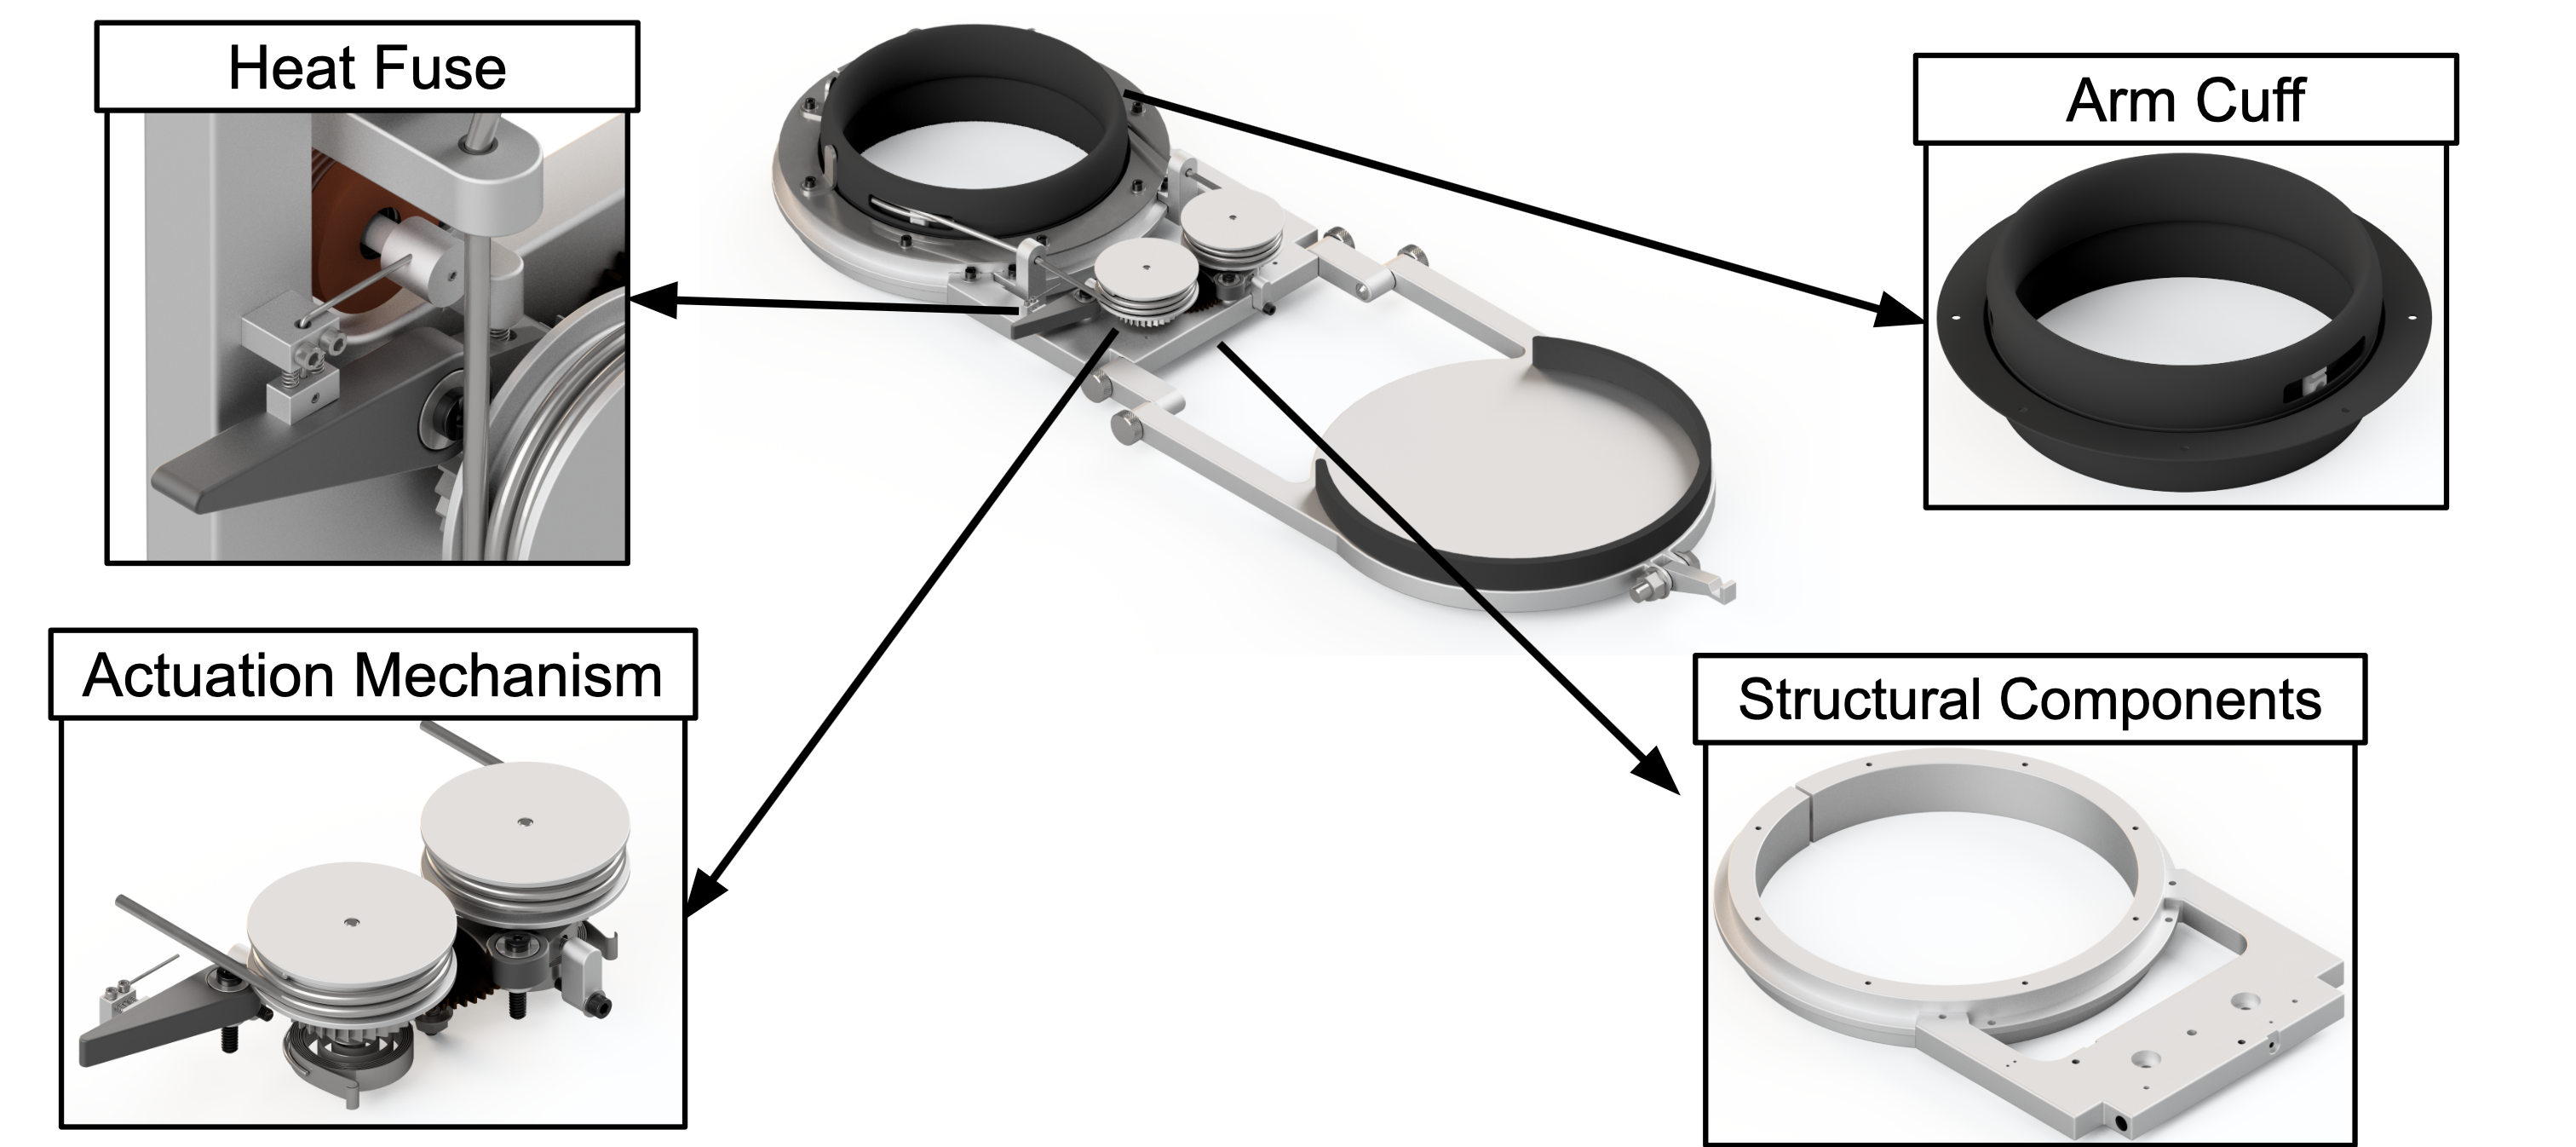
\includegraphics[width=1\linewidth]{Images/Instructional/Subsections.png}
    \caption{Subsections Overview}
    \label{fig:subsections}
\end{figure}

Figure \ref{fig:subsections}

\subsection{Arm Cuff}
The primary purpose of the arm cuff is to reduce the airflow into the glovebox from 90 CFM to 1 CFM. It is composed of three components, the outer wrap, the inner strip, and 8 clips which hold the cable.
\begin{itemize}
    \item Outer Wrap: Refrasil cloth intended to withstand 1700$^\circ$F temperatures and restrict airflow into Glovebox. 
    \item Inner Strip: Locates cloth clips. 
    \item Cloth clips: Guides cable wrap and distrubtes pressure around user arm during activation. 
\end{itemize}
\begin{figure}[H]
    \centering
    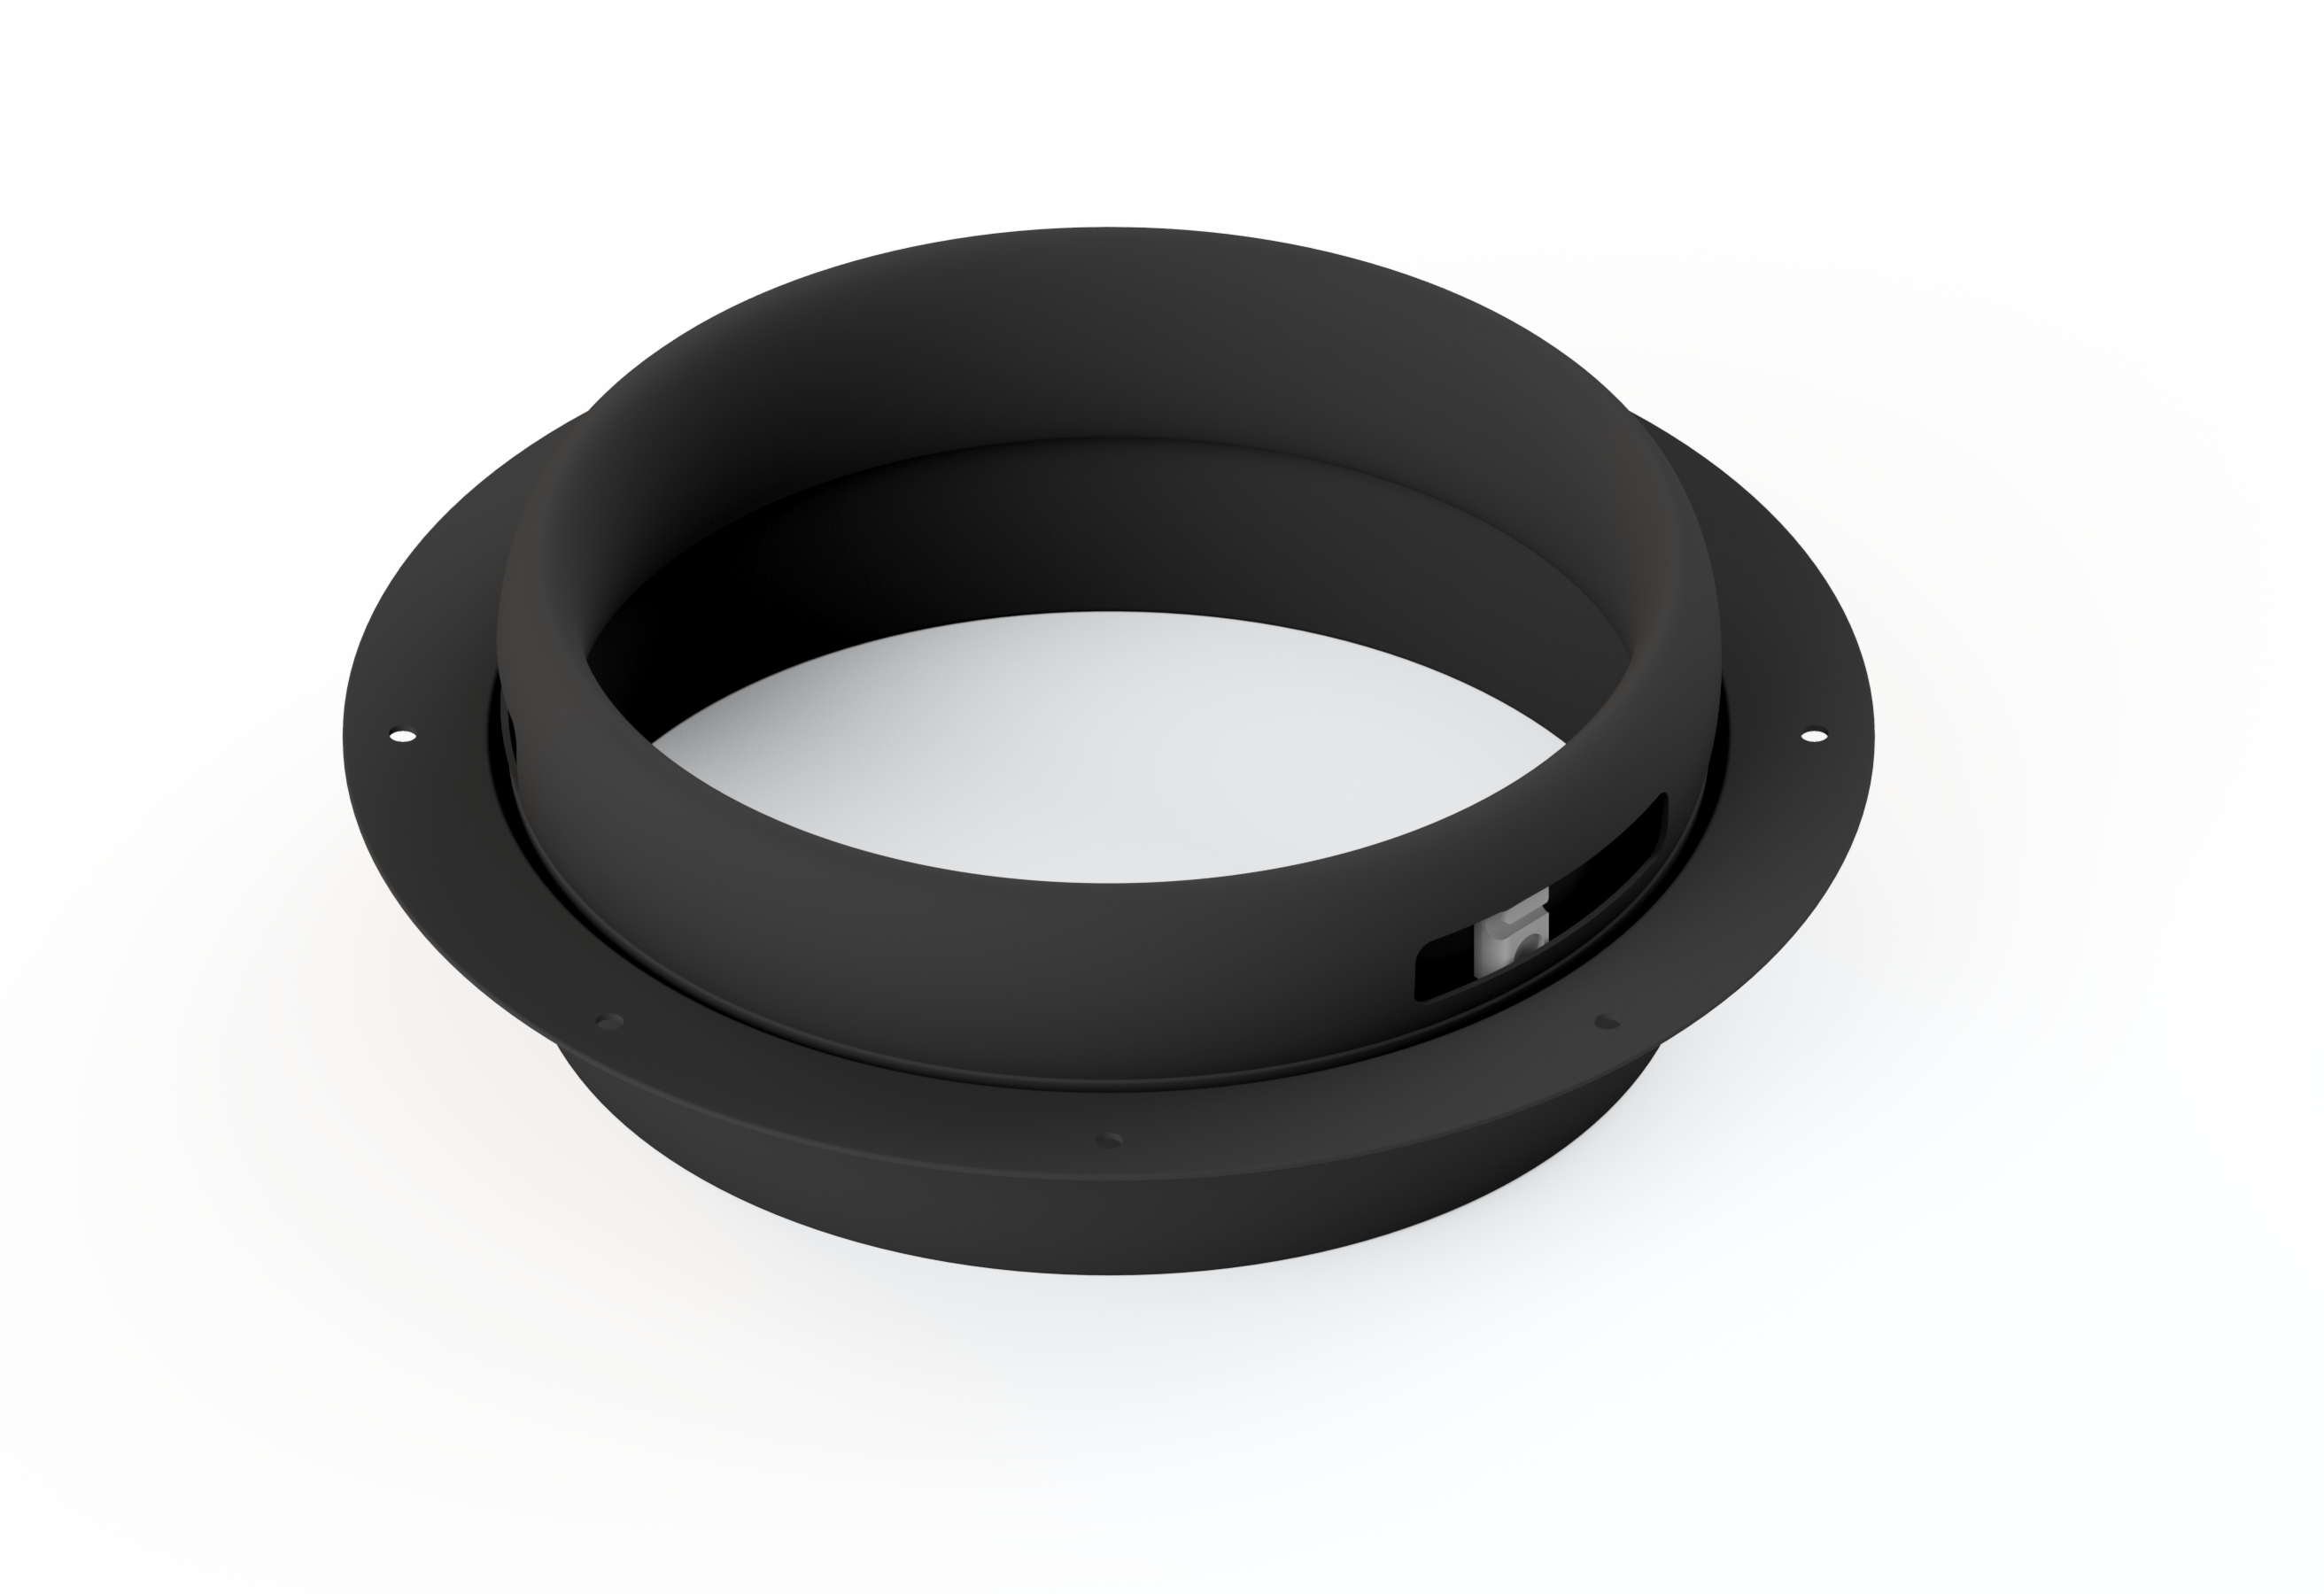
\includegraphics[width=0.45\linewidth]{Images/Arm Cuff/Pad (Open).png}
    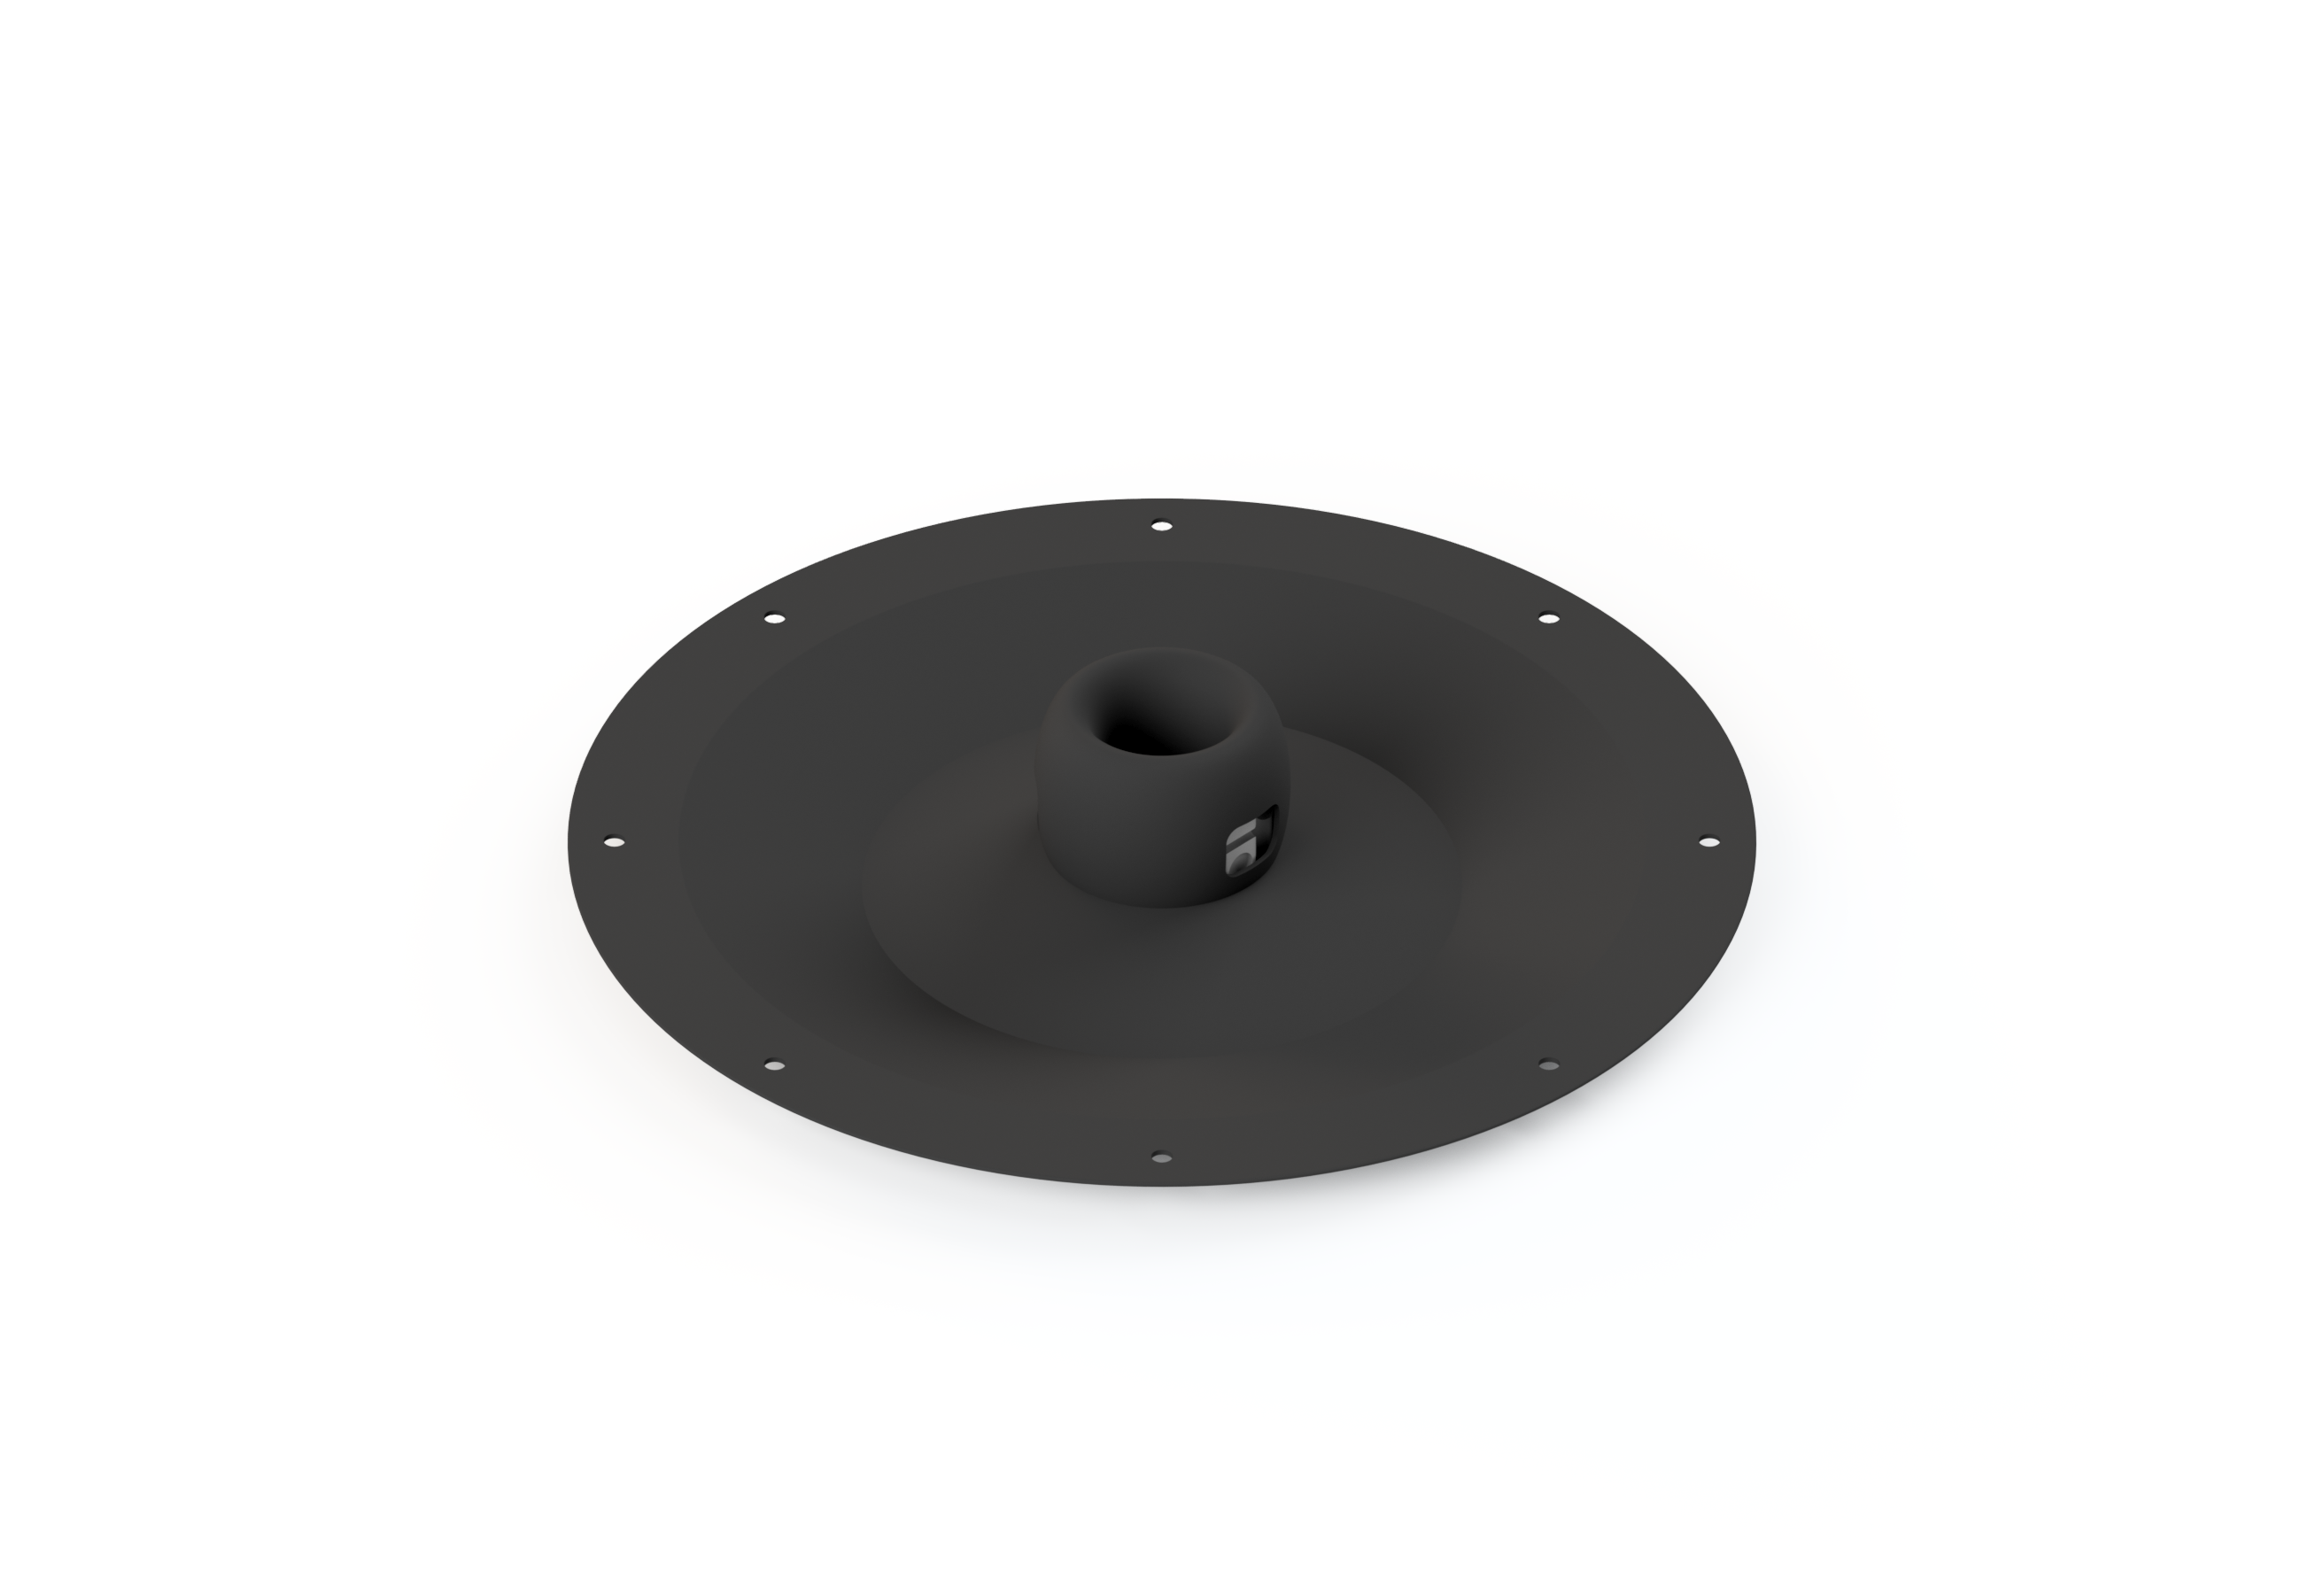
\includegraphics[width=0.45\linewidth]{Images/Arm Cuff/Pad (Closed).png}
    \caption{Arm Cuff (Open \& Closed)}
    \label{fig:placeholder}
\end{figure}
\begin{figure}[H]
    \centering
    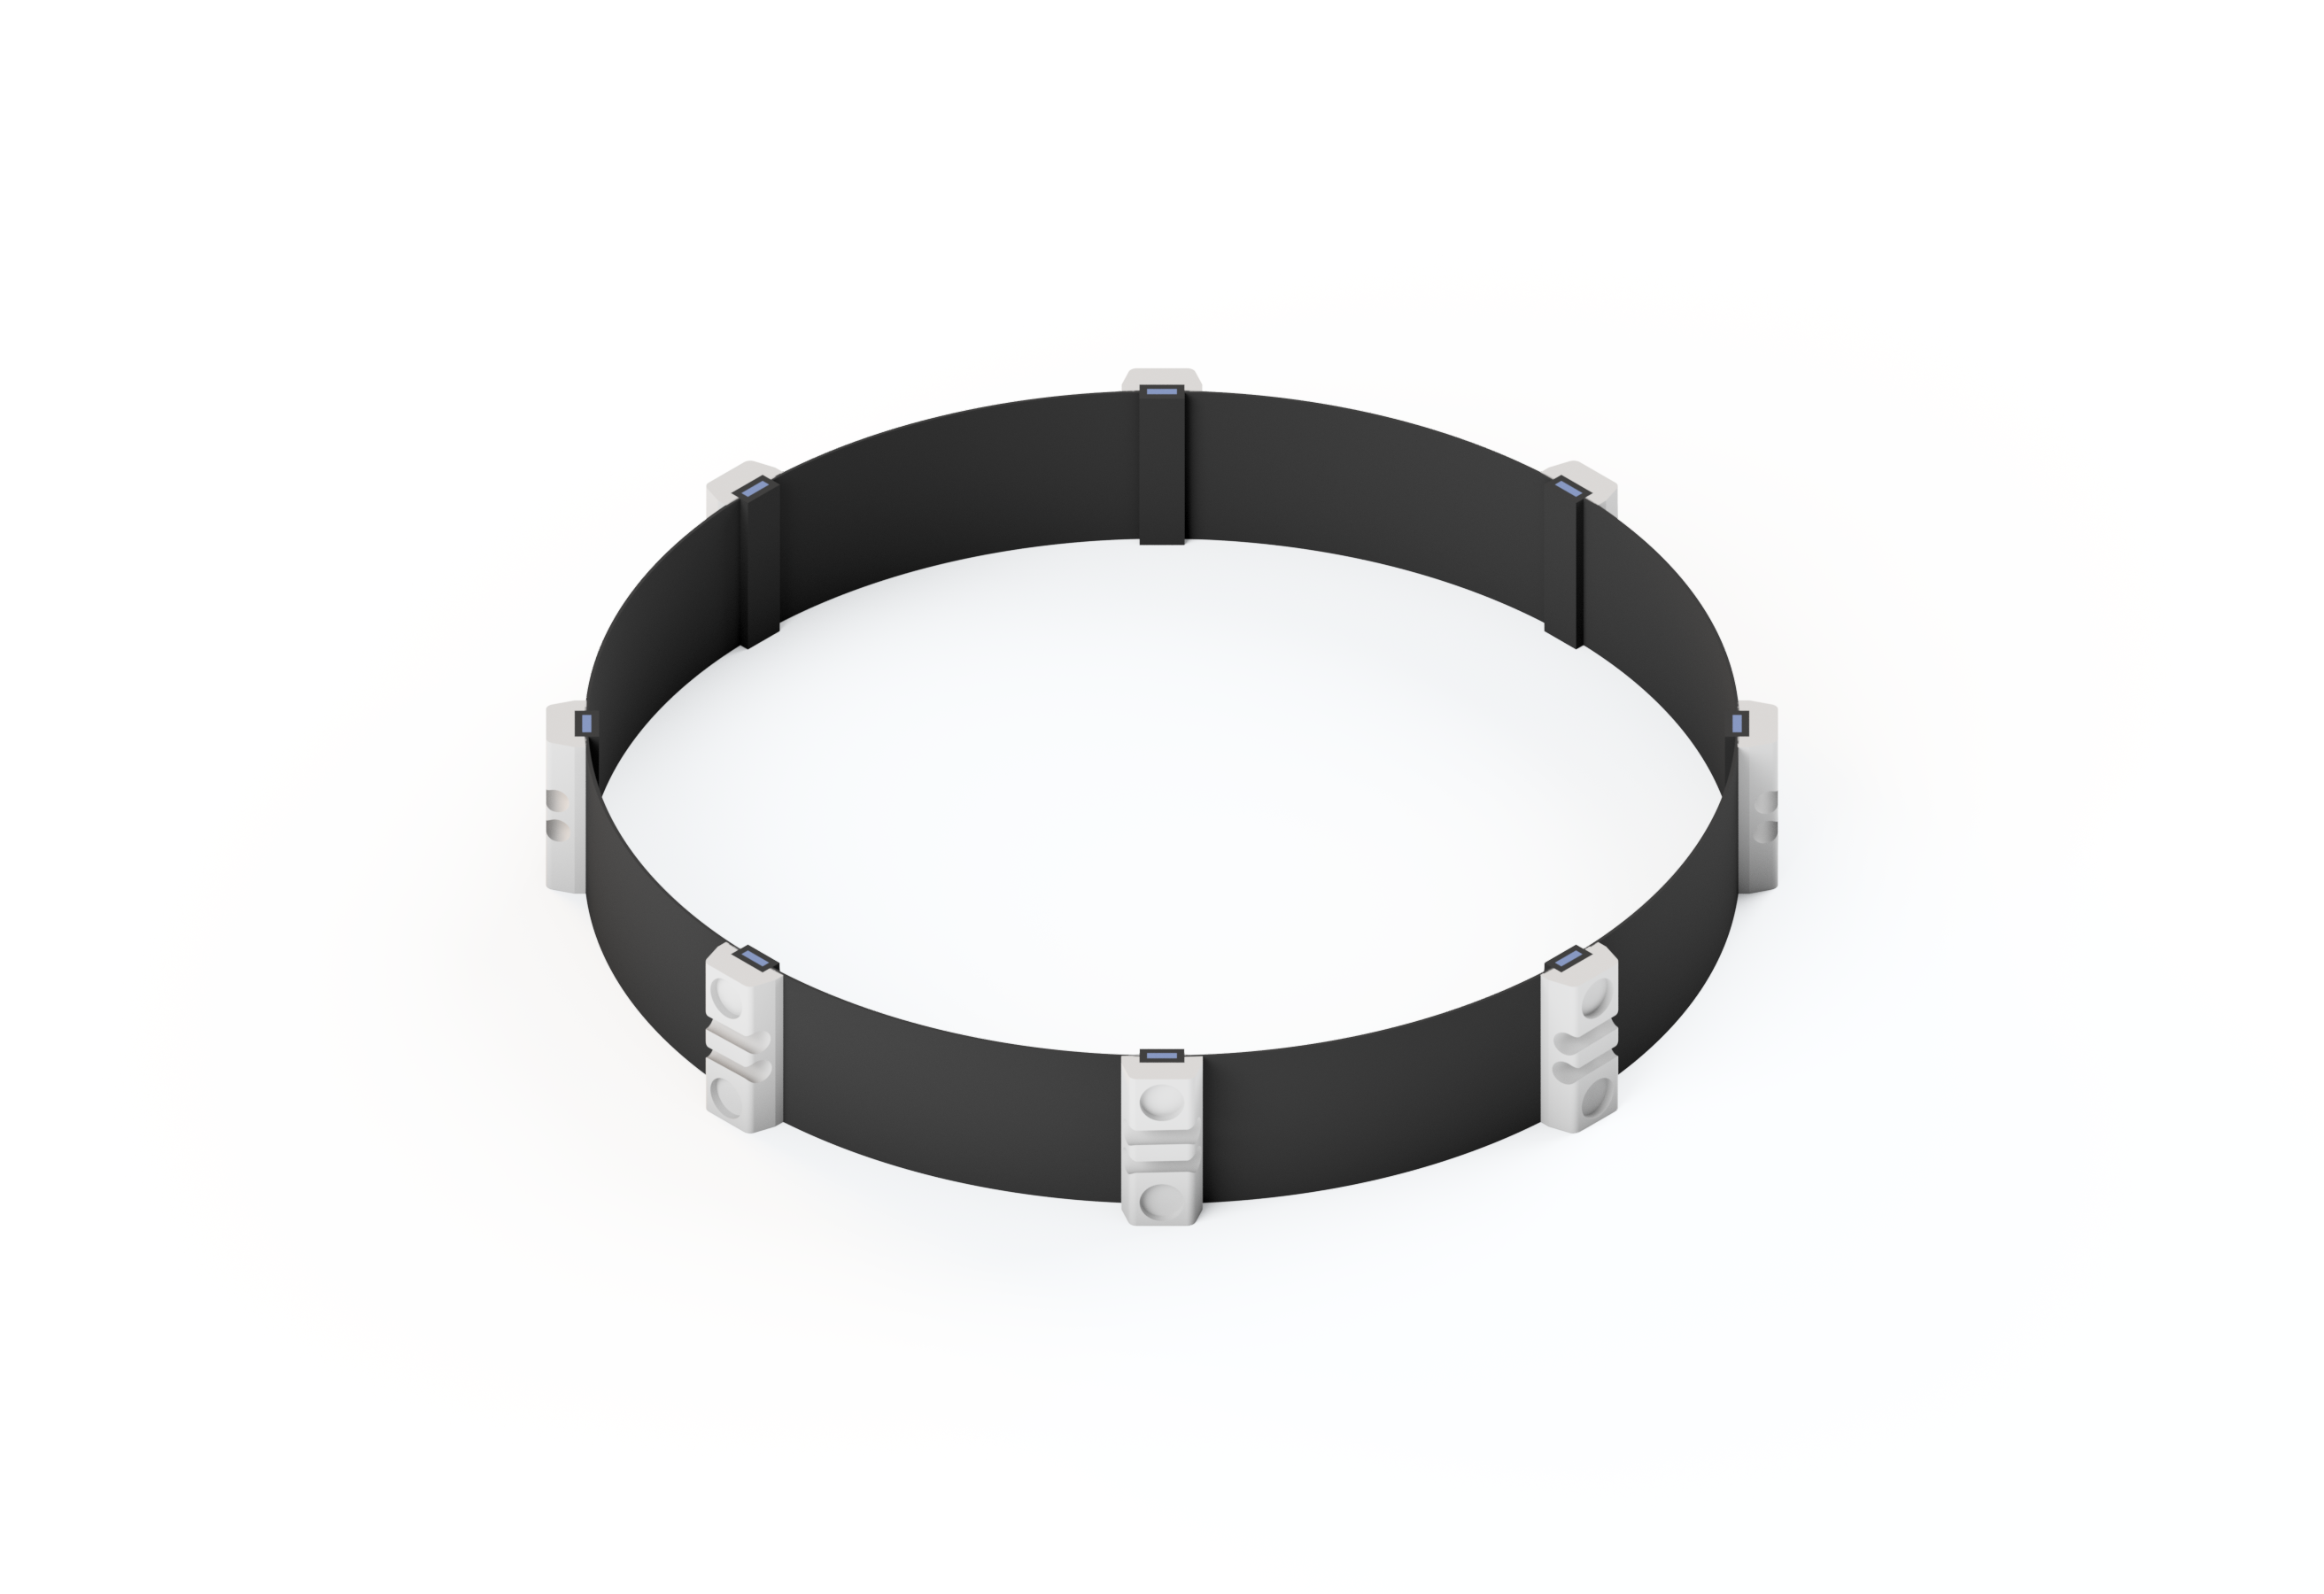
\includegraphics[width=0.45\linewidth]{Images/Arm Cuff/Pad (Clothless, Open).png}
    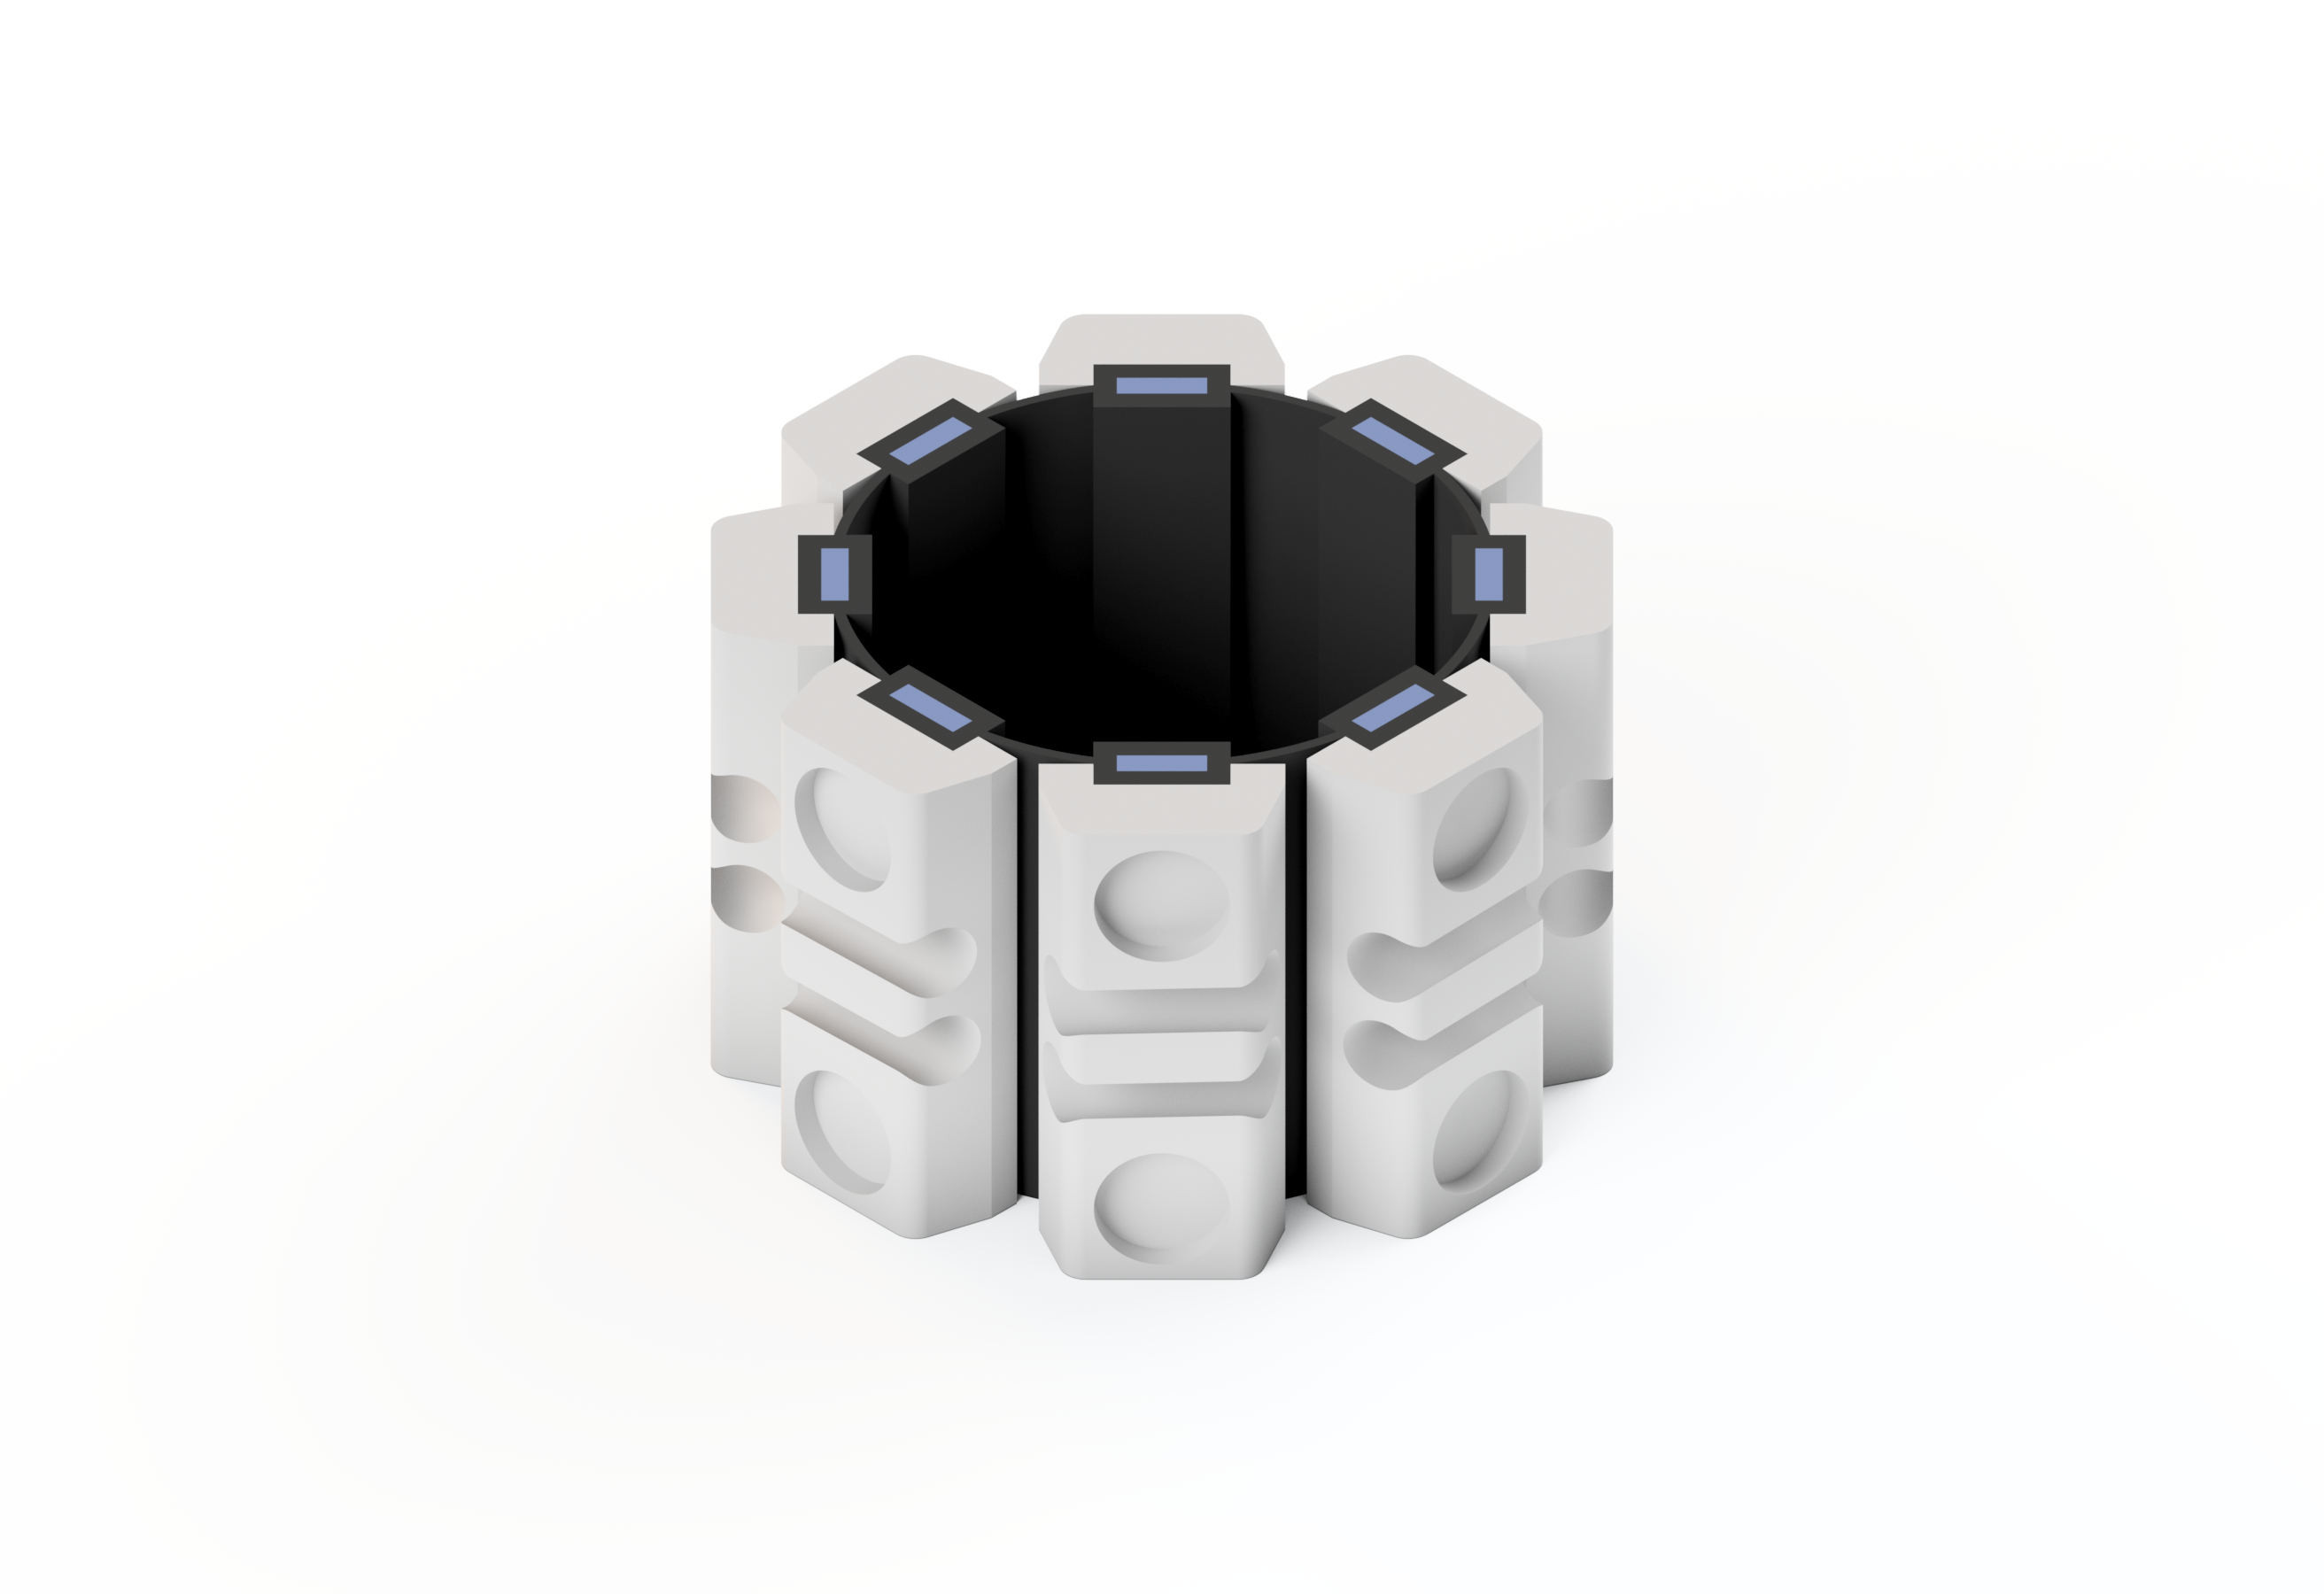
\includegraphics[width=0.45\linewidth]{Images/Arm Cuff/Pad (Clothless, Closed).png}
    \caption{Inner Strip with Clips (Open \& Closed)}
    \label{fig:placeholder}
\end{figure}

\subsection{Heat Fuse}
The heat fuse is what senses and initiates the mechanical motion of the closure mechanism. When the heat fuse reaches $180^\circ$F the small acrylic fuse will start to experience creep and allow the spring cable mechanism to actuate the lever.

\begin{figure}[H]
    \centering
    \includegraphics[width=0.45\linewidth]{Images/Heat Fuse/Heat Fuse Assembly.png}
    \caption{Heat Fuse Mechanism}
    \label{fig:placeholder}
\end{figure}
\begin{figure}[H]
    \centering
    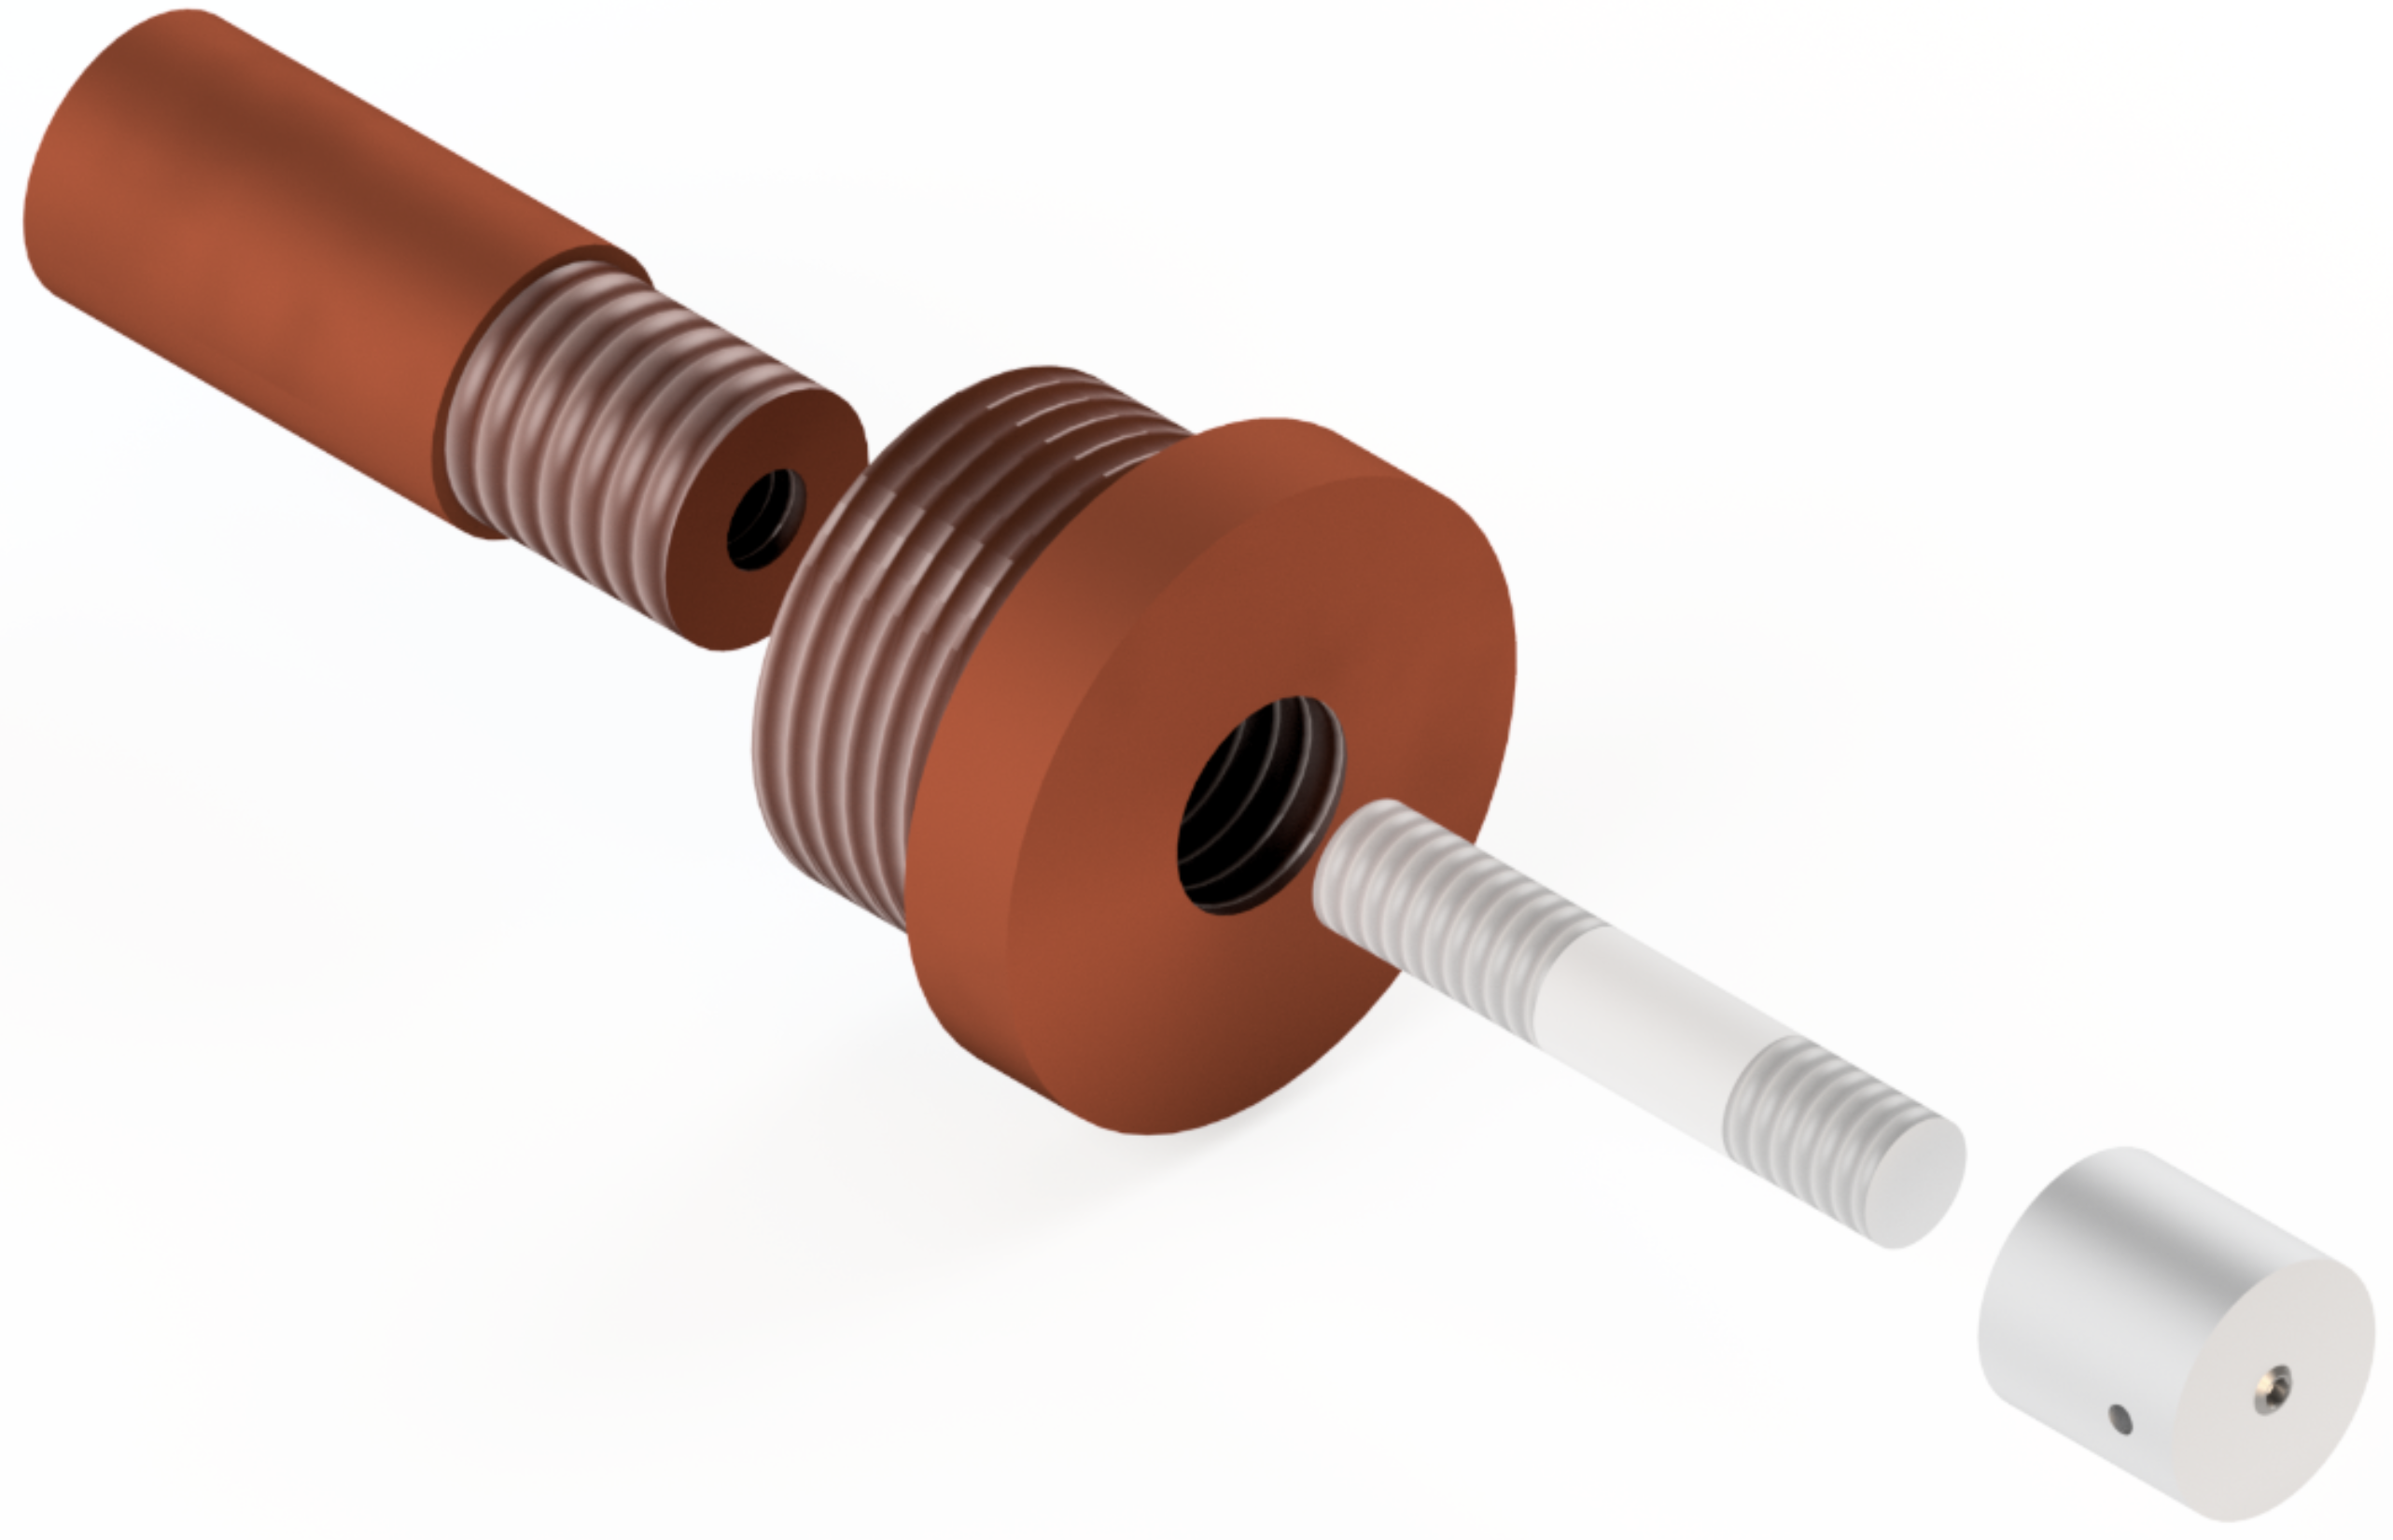
\includegraphics[width=0.45\linewidth]{Images/Heat Fuse/Heat Fuse Exploded.png}
    \caption{Heat Fuse Mechanism Exploded View}
    \label{fig:placeholder}
\end{figure}

\subsection{Actuation Mechanism}
The actuation mechanism is the mechanical component of the closure device, the main purpose is to draw in cable and in turn sinching the arm cuff. The activation mechanism is composed of two drums manipulated by rotor springs. The springs are located within the structural shelf and constrained by the rotor shaft, locator pins, and the steel cover plate (see \label{sec:Installation} ). The left drum serves as the primary actuator, upon release the left drum will draw in cable sinching the bag. The secondary (right) drum is on a mechanical delay using a 2:1 gear ratio, this allows the second spring to activate when the first one has drawn in the majority of the cable. The secondary spring ensures mechanism remains closed. 

The actuation mechanism can be manually operated with the lever on the left hand side. 

\begin{figure}[H]
    \centering
    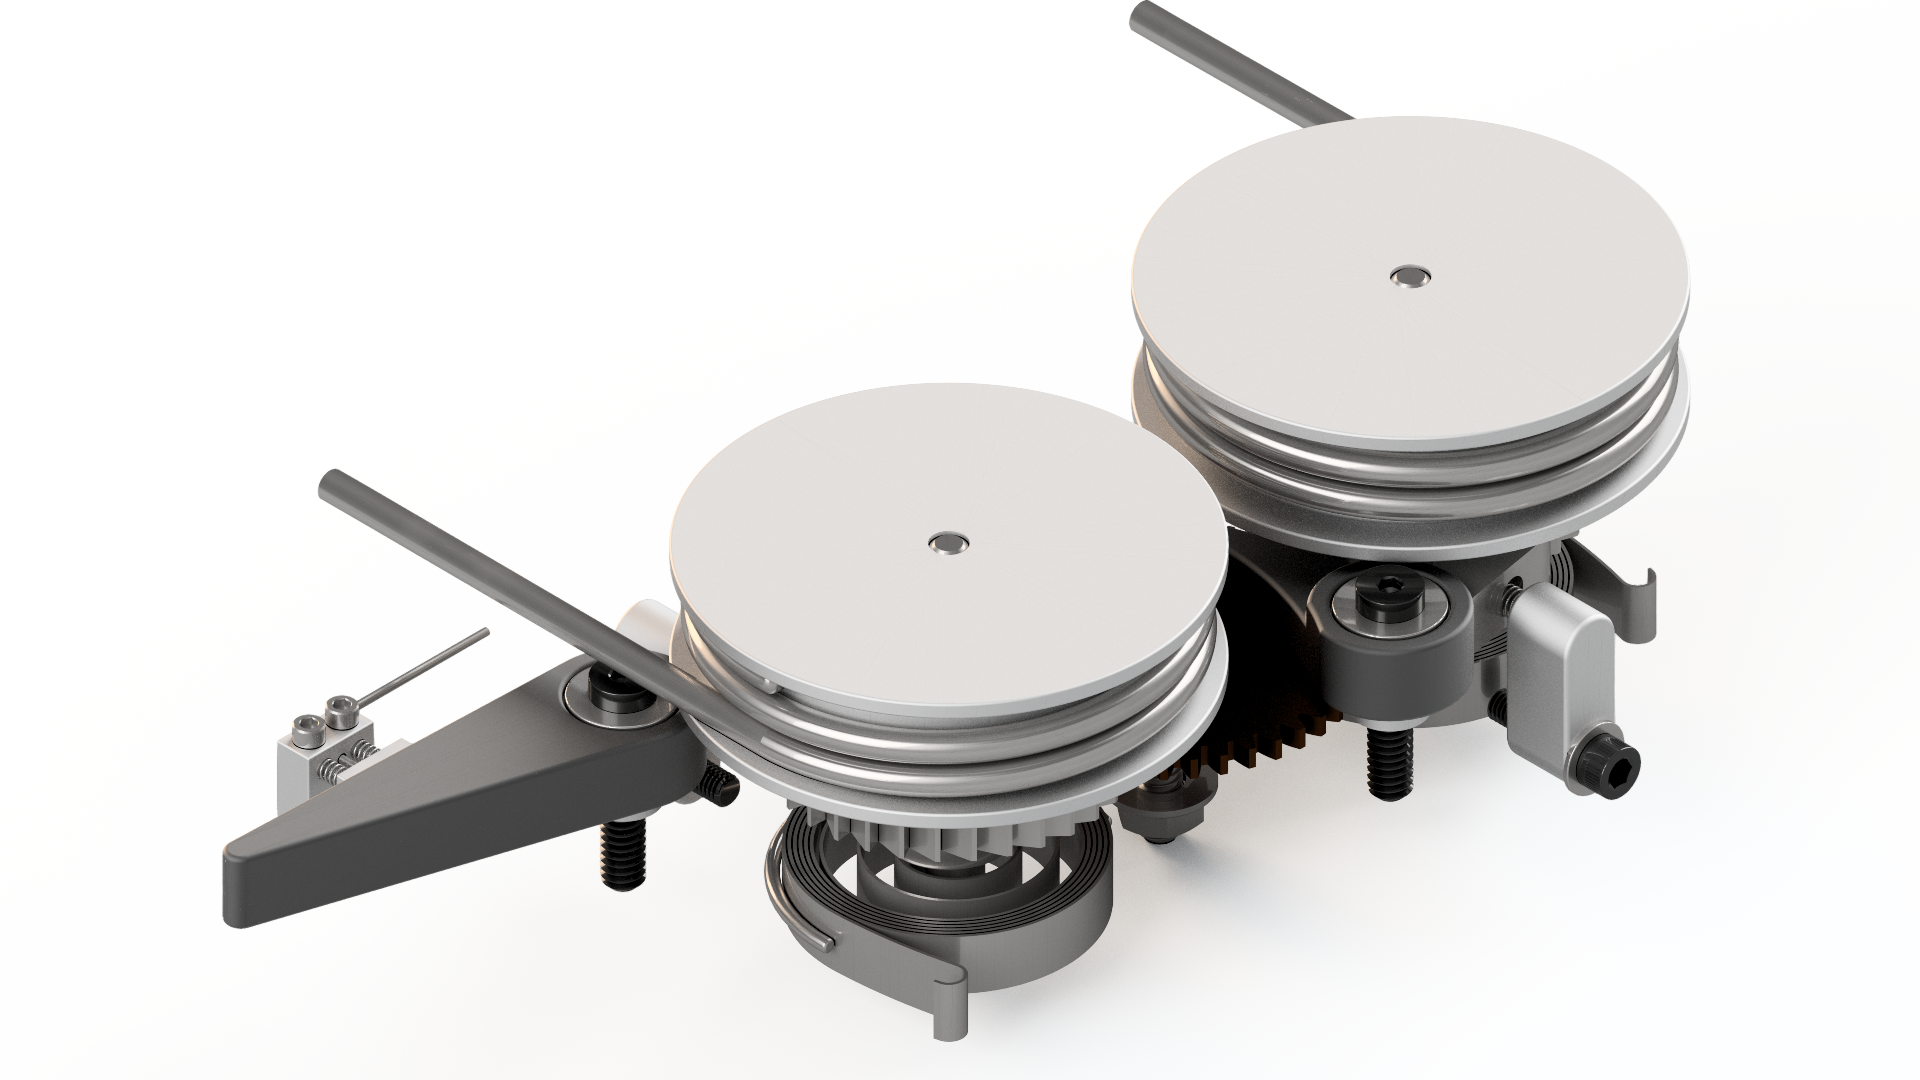
\includegraphics[width=0.45\linewidth]{Images/Actuation Mechanism/Mechanism Top.png}
    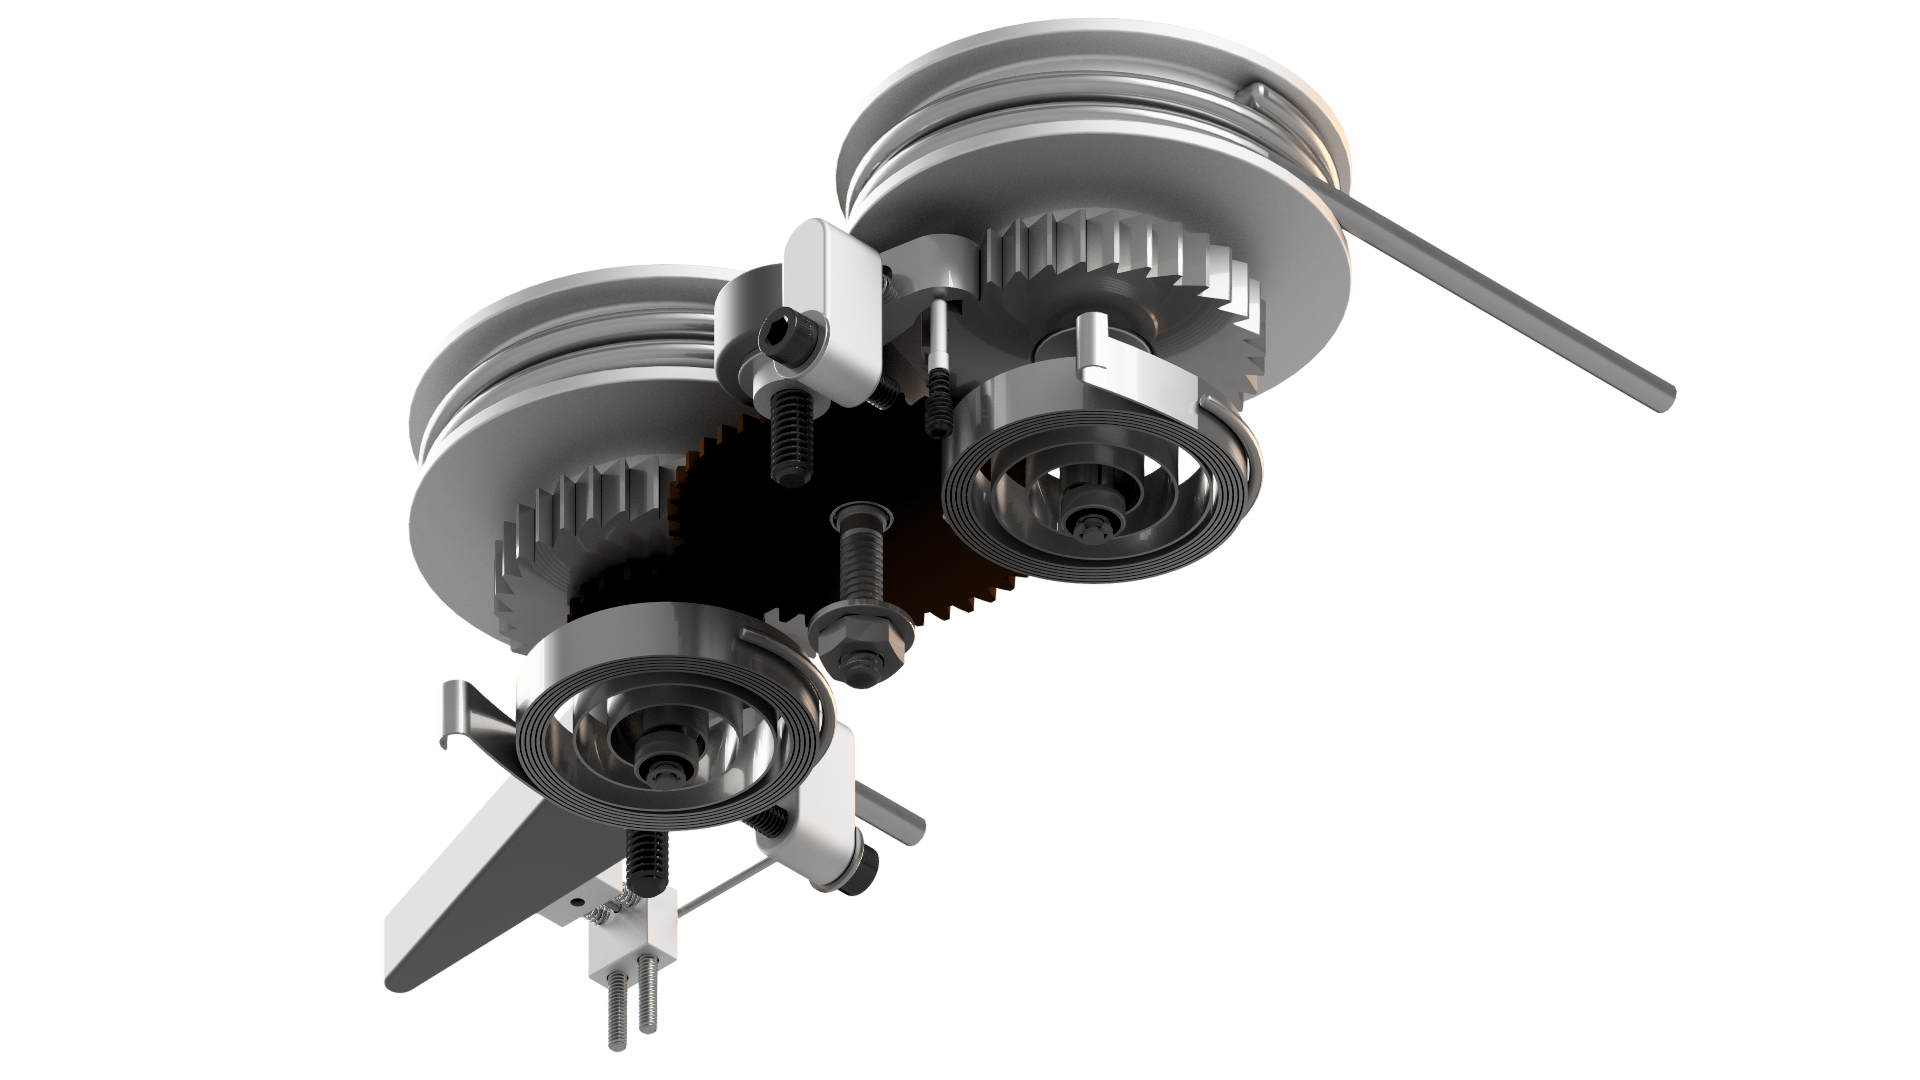
\includegraphics[width=0.45\linewidth]{Images/Actuation Mechanism/Mechanism Bottom.png}
    \caption{Actuation Mechanism (Top \& Bottom)}
    \label{fig:placeholder}
\end{figure}

\subsection{Secondary Closure}

The secondary closure device serves as a stationary air restriction that can be latched by the user. This closure flap must be manually manipulated by the user and should be used only when the user can do so safely. 
\begin{figure}[H]
    \centering
    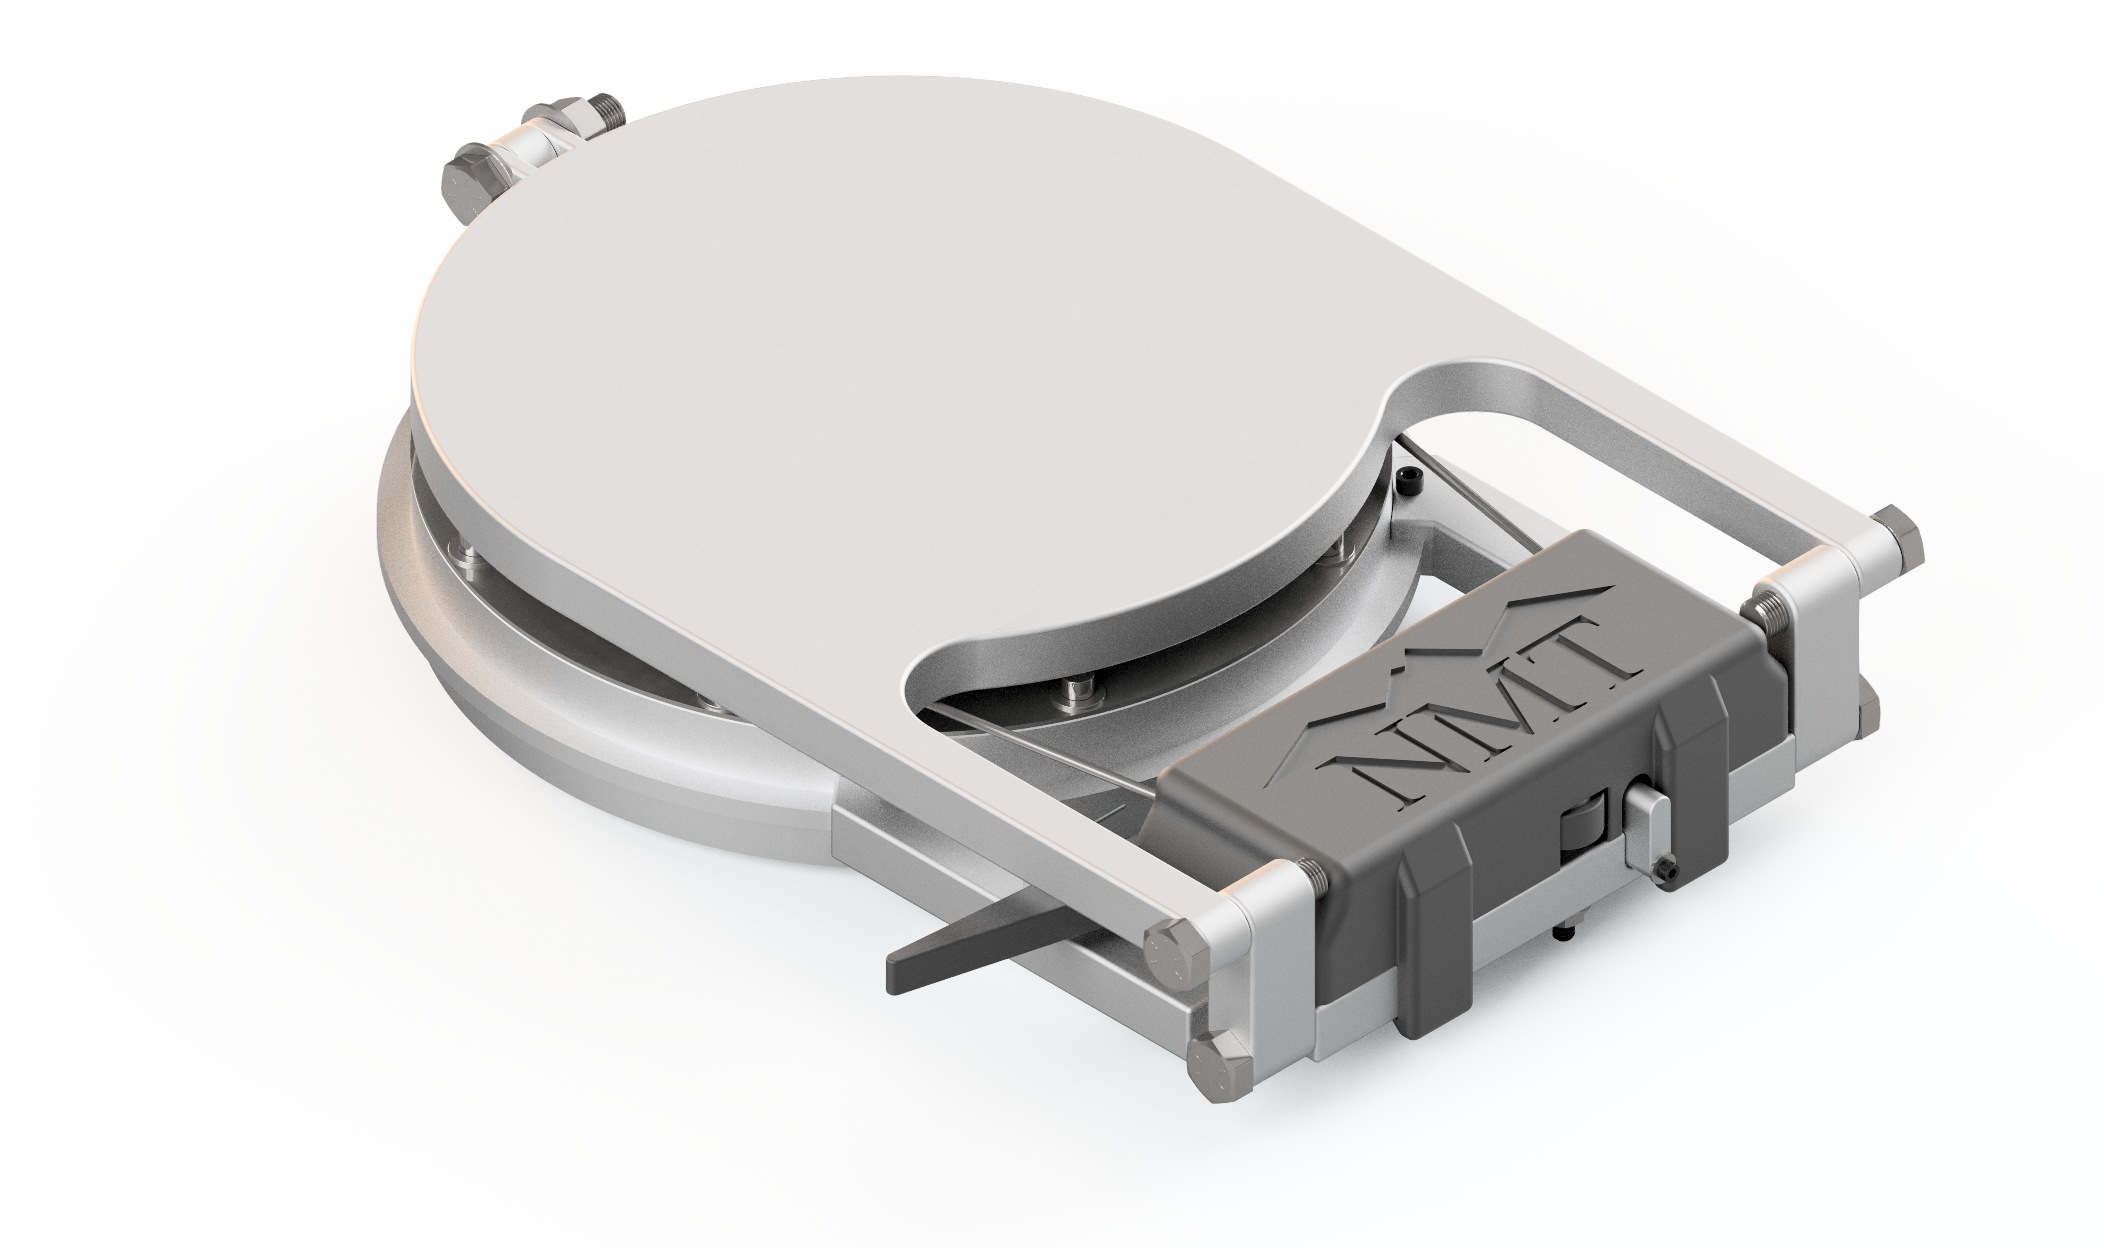
\includegraphics[width=0.45\linewidth]{Images/Secondary Closure/Closure Device (Covered, Secondary Closed).png}
    \caption{Secondary Closure Closed}
    \label{fig:placeholder}
\end{figure}

\begin{figure}[H]
    \centering
    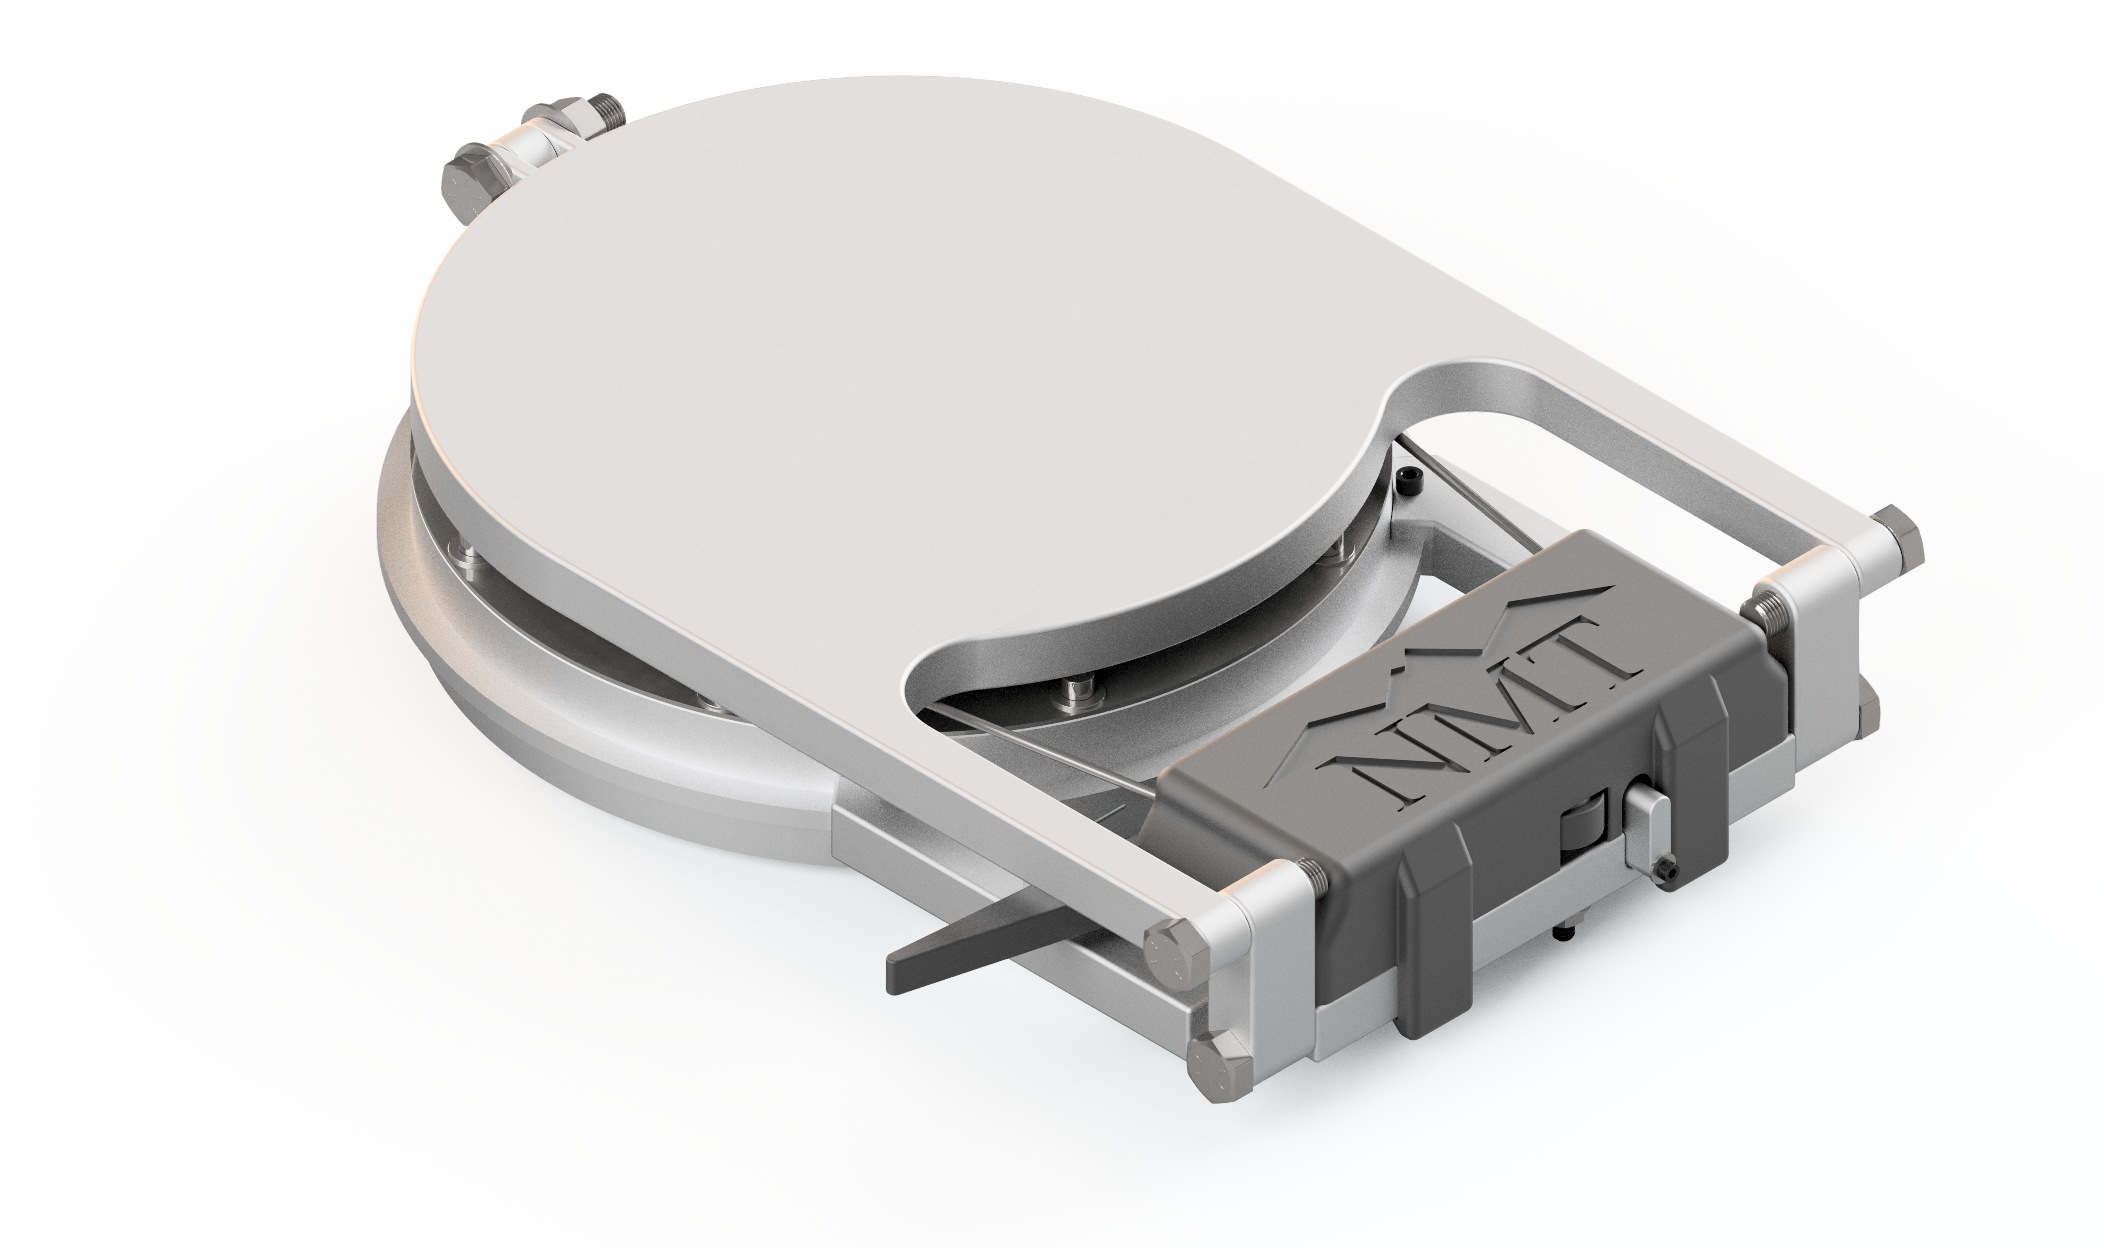
\includegraphics[width=0.45\linewidth]{Images/Secondary Closure/Closure Device (Covered, Secondary Closed).png}
    \caption{Secondary Closure Latch}
    \label{fig:placeholder}
\end{figure}

% Chapter 2: Safety Information
\chapter{Safety Information}

\section{General Safety Warnings}
    \begin{danger}
        Indicates a hazard that will result in death or serious injury.
    \end{danger}
    \begin{warning}
        Indicates a hazard that could result in death or serious injury.
    \end{warning}
    \begin{caution}
        Indicates a hazard that could result in a moderate or minor injury.
    \end{caution}
    \begin{notice}
        Indicates practical advice, or a situation that will result in damaged
        equipment.
    \end{notice}

\hline
   
    \begin{warning}
        This device is designed to actuate automatically when exposed to elevated temperatures associated with a fire. Users must not place hands, tools, or foreign objects within the path of the actuation mechanism while the device is armed. Sudden mechanical movement may occur when the thermal fuse activates.
    \end{warning}

    \begin{warning}
        The device contains springs, cables, and other mechanical parts that store potential energy when the system is armed. Improper handling during installation, maintenance, or reset procedures may result in sudden release of stored energy and potential injury.
    \end{warning}

    \begin{warning}
        This system is intended to supplement existing fire safety infrastructure. It is not designed to extinguish fires or replace fire suppression systems. Always follow established fire response procedures.
    \end{warning}

\section{Design Limitations}
    This device is designed to reduce airflow into the glovebox during elevated temperature events. It is not intended to fully seal the glovebox or provide containment of hazardous materials.

    The closure mechanism reduces the influx of oxygen into the glovebox during a fire event but does not eliminate airflow entirely. Additional safety systems, including fire suppression and facility safety procedures, must remain in place.

    The device is designed for operation within the specified temperature limits and mechanical loading conditions described in the technical specifications. Operation outside these limits may result in failure to actuate or unintended actuation.

    Unauthorized modification of the mechanism, including alterations to the spring system, actuation mechanism, thermal fuse, or closure materials, may compromise system functionality. 
    
\section{Intended Use}
    The intended use of this device is to reduce the airflow into a glovebox during a fire event or other high temperature event. The glovebox operates under negative pressure, which may draw external air into the enclosure when structural components fail or when gloves fail during elevated temperature events.

    The closure mechanism is designed to automatically deploy when the thermal fuse reaches its activation temperature. Upon activation, the actuation mechanism releases stored mechanical energy, allowing the closure system to tighten around the glove port opening and restrict incoming airflow.

    The device should only be used as part of a properly maintained glovebox system and must be installed according to the procedures described in this manual.
    
\section{Emergency Procedures}
    
    If the device activates during a fire event, personnel should immediately follow established emergency response procedures. Do not attempt to manually interfere with the closure mechanism during actuation.

    After activation, the device must be inspected before being returned to service. This includes verifying that the thermal fuse has been replaced, cables and springs remain intact, and that the actuation mechanism resets correctly.

    If the device fails to actuate during a fire event, personnel should follow standard fire response protocols and notify the responsible laboratory safety personnel. The device should be removed from service and inspected for mechanical failure or thermal fuse malfunction.

    Under no circumstances should the device be reset or repaired while the glovebox is in an unsafe condition.

% Chapter 3: Installation
\chapter{Installation}

\section{Inspection of Device}

Prior to installation of closure mechanism complete the following inspection checklist. 

\begin{enumerate}
    \item Ensure maintenance pin is inserted.
    \item Ensure device is unarmed. 
    \item Ensure rotor springs are undamaged and secure. 
    \begin{enumerate}
        \item Stand device up right with the ring pointing upwards. 
        \item Remove steel cover plate on back of device. 
        \item Inspect both rotor springs for damage. If damage is suspected do not install device. Report damage and replace springs. 
        \item Ensure outer spring tail is captured between shelf indent and pin. 
        \item Ensure inner spring tail is secure in the rotor shaft slot. 
        \item Reinstall cover plate ensuring pin alignment. 
        \item Lay device on it's back on a flat unobstructed surface. 
    \end{enumerate}
    \item Ensure secondary pawl latch is in the lowered position underneath the secondary pawl. The latch should not restrict the movement of the pawl. 
    \item Inspect spindle assembly. 
    \begin{enumerate}
        \item Inspect assemblies for visible damage or wear. 
        \item Ensure shafts are perpendicular to shelf face. 
        \item Inspect gears for misalignment. 
    \end{enumerate}
    \item Ensure the cable is wrapped around each drum about three times. 
    \item Inspect arm cuff for fabric damage. 
\end{enumerate}
\section{Mounting on Glovebox}
    \begin{enumerate}
        \item Ensure that maintenance pin is inserted and plastic covers are attached
        \item Slide device over the gloveport
        \item Tighten bolt at the top of the split colar
        \item Insert the heat fuse into the leftmost sensor port beneath the Glove port
        \item Attach the cable between the actuation spring and the Heat Fuse
        \item Remove the maintenance pin
    \end{enumerate}

\section{How to Arm the Device}
    \begin{enumerate}
        \item Ensure that the maintenance pin is not inserted under the actuation lever
        \item Wind the left drum
        \item Wind the right drum
        \item Attach cloth bag to the magnetic clips around the orafice
    \end{enumerate}

% Chapter 4: Operation
\chapter{Operation}

\section{Modes of Operation}
    \begin{itemize}
        \item \textbf{Standby:} System is armed and monitoring sensors.
        \item \textbf{Triggered:} Fire detected, mechanism closed.
        \item \textbf{Maintenance:} Actuation blocked by maintenance pin
    \end{itemize}
    
\subsection{Maintenance Mode}
To put the device in maintenance mode insert the pin as seen in the figure below. Once the pin is inserted the mechanism is unable to actuate. To take the device out of maintenance mode remove the pin.

% \begin{figure}[H]
%     \centering
%     \includegraphics[width=0.45\linewidth]{Images/Instructional/Maintenance Pin.png}
%     \caption{Maintenance Pin}
%     \label{fig:placeholder}
% \end{figure}

\section{Manual Operation}
To manually activate the device, push the lever on the left side of the device, it should immediately actuate. Manual activation does not trigger the heat fuse and does not require replacement. 

\section{Automatic Actuation (Fire Event)}
    \begin{enumerate}
        \item Fire starts inside glovebox
        \item Fire heats the heat fuse to $180^oF$
        \item Acrylic piece of the heat fuse melts and experiences creep
        \item Actuation lever is depressed by the heat fuse spring mechanism
        \item First drum rotates twice before actuating the second drum
        \item Drum rotation pulls on cable tightening bag and reducing airflow into the glovebox.
    \end{enumerate}

\section{Resetting After Trigger}
    \begin{caution}
        Do not reset the mechanism until the fire has been fully extinguished and the glovebox atmosphere is stable.
    \end{caution}

After the device has been activated during a fire event, the mechanism must be inspected and reset before it can be returned to service. \textbf{DO NOT INSPECT UNLESS GLOVEBOX HAS BEEN DEEMED SAFE BY THE APPROPRIATE PERSONNEL} Follow the procedure below to safely reset the device. 
    
    \begin{enumerate}
        \item 
    \end{enumerate}

% Chapter 5: Maintenance and Testing
\chapter{Maintenance and Testing}

\section{Routine Inspection Schedule}
    % Daily, Weekly, Monthly checks.
    
\section{Assembly Guide}

%All those other testing procedures

% Chapter 6: Troubleshooting
\chapter{Troubleshooting}
    \begin{table}[H]
        \centering
        \begin{tabular}{|p{4cm}|p{5cm}|p{5cm}|}
        \hline
        \textbf{Problem} & \textbf{Possible Cause} & \textbf{Solution} \\ \hline
        False Actuation & Broken Cable & Increase threshold or reposition sensor \\ \hline
        Mechanism Jams & Debris in track & Clean gears \\ \hline
        Mechanism Jams & Broken Springs & Replace Springs \\ \hline
        \end{tabular}
        \caption{Troubleshooting Guide}
    \end{table}

% Appendices
\appendix
\chapter{Technical Specifications}

\end{document}